%============================================================================%
% Antoine Géré (gereantoine@gmail.com).
% Presentation Ph.D. thesis. (2013--2015)
% Analytic regularization of quantum field theories on curved backgrounds.
% --
% Università degli Studi di Genova.
% http://www.unige.it
% --
% Dipartimento di Matematica,
% Via Dodecaneso 35, 16146 Genova, Italia.
%============================================================================%
% LaTeX environment, Kile : available at http://kile.sourceforge.net/
% --
% Package : available at http://www.ctan.org/
% --
% The comprehensive latex symbole list : available at http://www.ctan.org/tex-archive/info/symbols/comprehensive/
% Detexif (an attempt to simplify the search in the latex symbole list) : available at http://detexify.kirelabs.org/classify.html
% --
% Bibliography with Zotero : available at http://www.zotero.org/
% Bib style : http://arxiv.org/hypertex/bibstyles/
% --
% Latex font catalogue : available at http://www.tug.dk/FontCatalogue/
%============================================================================% 

\documentclass[9pt]{beamer}

%----------------------------------------------------------------------------%

\pdfoutput=1
\makeatletter

%----------------------------------------------------------------------------%

\usepackage{amscd}
\usepackage{amsmath}
\usepackage{amsthm}
\usepackage{amsxtra}
\usepackage{array} 
\usepackage[english]{babel} 
\usepackage{cancel}
\usepackage{color}
\usepackage{enumitem}
\usepackage{fancyhdr}
\usepackage{relsize}
\usepackage[T1]{fontenc} 
\usepackage{geometry} 
\usepackage{graphicx} 
\usepackage{hyperref} 
\usepackage[utf8]{inputenc} 
\usepackage{letltxmacro}
\usepackage{lmodern}
\usepackage{manfnt}
\usepackage{multicol} 
\usepackage[numbers,sort]{natbib}
\usepackage{pgf}
\usepackage{setspace} 
\usepackage{tikz}
\usepackage{url}
\usepackage{wasysym}
\usepackage{wrapfig}
\usepackage{xcolor}

%============================================================================%    

\mode<presentation>
{

%== NAVIGATION SYMBOLS ======================================================%    

\setbeamertemplate{navigation symbols}{}
  
%== TITLE PAGE ==============================================================%    

\newcommand\conference[1]{\def\insertconference{#1}}
\conference{}

\newcommand\shortconference[1]{\def\insertshortconference{#1}}
\shortconference{}

\newcommand\paper[1]{\def\insertpaper{#1}}
\paper{}

\newcommand\LogoUniv[1]{\def\insertLogoUniv{#1}}
\paper{}
  
\newcommand\TitlePic[1]{\def\insertTitlePic{#1}}
\paper{}

\pgfdeclareverticalshading[title page.bg]{beamer@titleshade}{\paperwidth}{%
color(0pt)=(black!30!white);
color(3pt)=(black!60!white);
color(3pt)=(title page.bg);
color(126pt)=(title page.bg);
color(126pt)=(black!60!white);
color(129pt)=(black!30!white)}
 
\defbeamertemplate*{title page}{gottingen14}[1][]
{%
\hbox{%
%
\leavevmode%
\advance\beamer@leftmargin by -12bp%
\advance\beamer@rightmargin by -12bp%
\beamer@tempdim=\textwidth%
\advance\beamer@tempdim by \beamer@leftmargin%
\advance\beamer@tempdim by \beamer@rightmargin%
\hskip-\Gm@lmargin%
%
\hbox{%
\setbox%
\beamer@tempbox=\hbox{%
%
\begin{minipage}[b]{\paperwidth}%
\vbox{}%
\leavevmode%
\center{%
{\usebeamerfont{title}\inserttitle} \\[4pt]
{\usebeamerfont{author}\color{black}\insertauthor}\\[1pt]%
%\insertLogoUniv
{\color{black}\insertdate}\\
{\usebeamerfont{conference}\color{black}\insertconference}\\[-2pt]%
{\usebeamerfont{institute}\color{black}\insertinstitute}\\[-6pt]
}%
\strut%
\par%
\vbox{}%
\end{minipage}%
}%
%
\beamer@tempdim=\ht\beamer@tempbox%
\advance\beamer@tempdim by 115pt%
%
\begin{pgfpicture}{0pt}{0pt}{\paperwidth}{\beamer@tempdim}
\pgfsetfillopacity{0.8}
\pgftext[left,base]{\pgfuseshading{beamer@titleshade}}
\end{pgfpicture}
%
\hskip-\paperwidth%
\box\beamer@tempbox%
}%
}%
}

%== TEMPLATE ================================================================% 
 
\setbeamertemplate{title page}[gottingen14][colsep=-4bp,rounded=false]
\setbeamertemplate{sections/subsections in toc}[ball]
\setbeamertemplate{items}[ball]
\setbeamertemplate{blocks}[default]
\setbeamertemplate{part page}[default][colsep=-4bp,rounded=false]
    
%== COLOR ===================================================================% 
  
\setbeamercolor{title page}{bg=white!96!black,fg=red!62!black}
\setbeamercolor{frametitle}{bg=white,fg=red!60!black}
\setbeamercolor{subsection in head/foot}{bg=white!95!black,fg=red!60!black}
\setbeamercolor{author in head/foot}{bg=white,fg=red!60!black}
\setbeamercolor{title in head/foot}{bg=white,fg=red!60!black}
\setbeamercolor{normal text}{black}
\setbeamercolor{headline@color}{bg=black,fg=green}
\setbeamercolor{block title}{bg=black!20!white,fg=red!60!black}
\setbeamercolor{block body}{bg=black!20!white,fg=black}
\setbeamercolor{block body alerted}{bg=black!40!white,fg=black}
\setbeamercolor{block title alerted}{bg=black!40!white,fg=black}
\setbeamercolor{block body example}{bg=black!10!white,fg=black}
\setbeamercolor{block title example}{bg=black!10!white,fg=red!60!black}
\setbeamercolor{button}{bg=black!50!white,fg=white}
\setbeamercolor{sidebar}{bg=black,fg=white}
\setbeamercolor{palette sidebar primary}{bg=black,fg=white}
\setbeamercolor{palette sidebar secondary}{bg=black,fg=white}
\setbeamercolor{palette sidebar tertiary}{bg=black,fg=white}
\setbeamercolor{palette sidebar quaternary}{bg=black,fg=white}
\setbeamercolor{titlelike}{bg=green,fg=white}
\setbeamercolor{separation line}{white}
\setbeamercolor{fine separation line}{white}

%== FONT ====================================================================% 
  
\setbeamerfont{frametitle}{size={\normalsize},series={\bf}}
\setbeamerfont{block title}{size={},series={}}
\setbeamerfont{block body}{size={},series={}}
\setbeamerfont{block title example}{size={},series={}}
\setbeamerfont{block body example}{size={},series={}}
\setbeamerfont{title}{size={\LARGE},series={\bf}}
\setbeamerfont{subtitle}{size={\large},series={\bf}}
\setbeamerfont{author}{size={\Large},series={\bf}}
\setbeamerfont{institute}{size={\normalsize},series={}}
\setbeamerfont{conference}{size={\large},series={}}
\setbeamerfont{date}{size={\normalsize},series={}}
\setbeamerfont{coauthor}{size={\normalsize},series={\bf}}
\setbeamerfont{paper}{size={\normalsize},series={\tt}}

%== COVERED =================================================================% 
  
\setbeamercovered{transparent}
   
%== SHADOWS =================================================================% 

\AtBeginDocument{%
\pgfdeclareverticalshading{beamer@topshade}{\paperwidth}{%
color(0pt)=(bg);%
color(4pt)=(black!50!bg)}%
\pgfdeclareverticalshading{beamer@bottomshade}{\paperwidth}{%
color(0pt)=(black!50!bg);%
color(4pt)=(bg)}%
\pgfdeclarehorizontalshading{beamer@rightshade}{\paperwidth}{%
color(0pt)=(black!50!bg);%
color(4pt)=(bg)}%
\pgfdeclarehorizontalshading{beamer@leftshade}{\paperwidth}{%
color(0pt)=(black!50!bg);%
color(4pt)=(bg)}%
}%

%== FRAME TITLE =============================================================% 

\pgfdeclareverticalshading[frametitle.bg]{beamer@frametitleshade}{\paperwidth}
{%
color(0pt)=(frametitle.bg);
color(36pt)=(frametitle.bg)
}%

\defbeamertemplate*{frametitle}{nosplit theme}
{%
\nointerlineskip%
\vskip-2.5pt%
\hbox{\leavevmode
\advance\beamer@leftmargin by -12bp%
\advance\beamer@rightmargin by -12bp%
\beamer@tempdim=\textwidth%
\advance\beamer@tempdim by \beamer@leftmargin%
\advance\beamer@tempdim by \beamer@rightmargin%
\hskip-\Gm@lmargin\hbox{%
\setbox\beamer@tempbox=\hbox{
\begin{minipage}[b]{\paperwidth}%
\vbox{}%
\vskip0ex%
\leftskip0.3cm%
\rightskip0.3cm plus1fil\leavevmode
\insertframetitle%
\ifx\insertframesubtitle\@empty%
\strut\par%
\else
\par{\usebeamerfont*{framesubtitle}{\insertframesubtitle}\strut\par}%
\fi%
\vskip5pt%
\nointerlineskip
\vbox{}%
\end{minipage}}%
\beamer@tempdim=\ht\beamer@tempbox%
\advance\beamer@tempdim by 2pt%
\begin{pgfpicture}{0pt}{0pt}{\paperwidth}{\beamer@tempdim}
\usebeamercolor{frametitle}
\pgfpathrectangle{\pgfpointorigin}{\pgfpoint{\paperwidth}{\beamer@tempdim}}
\pgfusepath{clip}
\pgftext[left,base]{\pgfuseshading{beamer@frametitleshade}}
\end{pgfpicture}
\hskip-\paperwidth%
\box\beamer@tempbox%
}%
\hskip-\Gm@rmargin%
}%
\nointerlineskip
\vskip-0.2pt
\hbox to\textwidth{\hskip-\Gm@lmargin\pgfuseshading{beamer@topshade}\hskip-\Gm@rmargin}
\vskip-2pt
}

%== FOOTLINE ================================================================%    

\newcommand{\backupbegin}{
\newcounter{framenumberappendix}
\setcounter{framenumberappendix}{\value{framenumber}}
}

\newcommand{\backupend}{
\addtocounter{framenumberappendix}{-\value{framenumber}}
\addtocounter{framenumber}{\value{framenumberappendix}} 
}

\defbeamertemplate*{footline}{nosplit theme}{%
\vskip1pt
\pgfuseshading{beamer@bottomshade}
\vskip1.5pt
\leavevmode%
\hbox{%
\begin{beamercolorbox}[wd=0.95\paperwidth,right]{footline@color}%
\insertframenumber{} / \inserttotalframenumber 
\end{beamercolorbox}%
}%
\vskip0.5pt%
}%
%
}%
%
\mode%
%
<all>

%----------------------------------------------------------------------------%

\newcommand{\sm}[1]{\left\langle #1 \right\rangle}
\newcommand{\abs}[1]{\left|{#1}\right|}
\newcommand{\norm}[1]{\left|{#1}\right|}
\renewcommand{\exp}{\mathsf{exp}}
\renewcommand{\log}{\mathsf{log}}
\newcommand{\alphabd}{\boldsymbol{\alpha}}
\newcommand{\betabd}{\boldsymbol{\beta}}
\renewcommand{\inf}{\mathsf{inf}}
\newcommand{\MS}{\mathbf{MS}}
\newcommand{\ms}{\mathsf{ms}}
\renewcommand{\sup}{\mathsf{sup}}
\renewcommand{\Re}{\mathsf{Re}}
\renewcommand{\Im}{\mathsf{Im}}
\newcommand{\pp}{\mathsf{pp}}
\newcommand{\loc}{\mathsf{loc}}
\newcommand{\rp}{\mathsf{rp}}
\newcommand{\pv}{\mathsf{pv}}
\renewcommand{\det}{\mathsf{det}}
\newcommand{\tr}{\mathsf{Tr}}
\newcommand{\WF}{\mathsf{WF}}
\newcommand{\supp}{\mathsf{supp}}
\newcommand{\sd}{\mathsf{sd}} 
\renewcommand{\div}{\mathsf{div}}
\newcommand{\exte}[1]{\overset{\circ}{#1}}
\newcommand{\reg}{\mathsf{reg}} 
\newcommand{\citebeam}[1]{\textit{\textcolor{black!60!white}{[#1]}}}
\renewcommand{\paper}[6]{#1, ``#2'', \href{#4}{arxiv: #3}, \href{http://dx.doi.org/#6}{#5}.}

%----------------------------------------------------------------------------%

\newcommand{\Acal}{\mathcal{A}}
\newcommand{\Bcal}{\mathcal{B}}
\newcommand{\Ccal}{\mathcal{C}}
\newcommand{\Dcal}{\mathcal{D}}
\newcommand{\Ecal}{\mathcal{E}}
\newcommand{\Fcal}{\mathcal{F}}
\newcommand{\Gcal}{\mathcal{G}}
\newcommand{\Hcal}{\mathcal{H}}
\newcommand{\Ical}{\mathcal{I}}
\newcommand{\Jcal}{\mathcal{J}}
\newcommand{\Kcal}{\mathcal{K}}
\newcommand{\Lcal}{\mathcal{L}}
\newcommand{\Mcal}{\mathcal{M}}
\newcommand{\Ncal}{\mathcal{N}}
\newcommand{\Ocal}{\mathcal{O}}
\newcommand{\Pcal}{\mathcal{P}}
\newcommand{\Qcal}{\mathcal{Q}}
\newcommand{\Rcal}{\mathcal{R}}
\newcommand{\Scal}{\mathcal{S}}
\newcommand{\Tcal}{\mathcal{T}}
\newcommand{\Ucal}{\mathcal{U}}
\newcommand{\Vcal}{\mathcal{V}}
\newcommand{\Wcal}{\mathcal{W}}
\newcommand{\Xcal}{\mathcal{X}}
\newcommand{\Ycal}{\mathcal{Y}}
\newcommand{\Zcal}{\mathcal{Z}}

%----------------------------------------------------------------------------%

\newcommand{\Abb}{\mathbb{A}}
\newcommand{\Bmbb}{\mathbb{B}}
\newcommand{\Cbb}{\mathbb{C}}
\newcommand{\Dbb}{\mathbb{D}}
\newcommand{\Ebb}{\mathbb{E}}
\newcommand{\Fbb}{\mathbb{F}}
\newcommand{\Gbb}{\mathbb{G}}
\newcommand{\Hbb}{\mathbb{H}}
\newcommand{\Ibb}{\mathbb{I}}
\newcommand{\Jbb}{\mathbb{J}}
\newcommand{\Kbb}{\mathbb{K}}
\newcommand{\Lbb}{\mathbb{L}}
\newcommand{\Mbb}{\mathbb{M}}
\newcommand{\Nbb}{\mathbb{N}}
\newcommand{\Obb}{\mathbb{O}}
\newcommand{\Pbb}{\mathbb{P}}
\newcommand{\Qbb}{\mathbb{Q}}
\newcommand{\Rbb}{\mathbb{R}}
\newcommand{\Sbb}{\mathbb{S}}
\newcommand{\Tbb}{\mathbb{T}}
\newcommand{\Ubb}{\mathbb{U}}
\newcommand{\Vbb}{\mathbb{V}}
\newcommand{\Wbb}{\mathbb{W}}
\newcommand{\Xbb}{\mathbb{X}}
\newcommand{\Ybb}{\mathbb{Y}}
\newcommand{\Zbb}{\mathbb{Z}}

%----------------------------------------------------------------------------%

\newcommand{\Arak}{\mathfrak{A}}
\newcommand{\Brak}{\mathfrak{B}}
\newcommand{\Crak}{\mathfrak{C}}
\newcommand{\Drak}{\mathfrak{D}}
\newcommand{\Erak}{\mathfrak{E}}
\newcommand{\Frak}{\mathfrak{F}}
\newcommand{\Grak}{\mathfrak{G}}
\newcommand{\Hrak}{\mathfrak{H}}
\newcommand{\Irak}{\mathfrak{I}}
\newcommand{\Jrak}{\mathfrak{J}}
\newcommand{\Krak}{\mathfrak{K}}
\newcommand{\Lrak}{\mathfrak{L}}
\newcommand{\Mrak}{\mathfrak{M}}
\newcommand{\Nrak}{\mathfrak{N}}
\newcommand{\Orak}{\mathfrak{O}}
\newcommand{\Prak}{\mathfrak{P}}
\newcommand{\Qrak}{\mathfrak{Q}}
\newcommand{\Rrak}{\mathfrak{R}}
\newcommand{\Srak}{\mathfrak{S}}
\newcommand{\Trak}{\mathfrak{T}}
\newcommand{\Urak}{\mathfrak{U}}
\newcommand{\Vrak}{\mathfrak{V}}
\newcommand{\Wrak}{\mathfrak{W}}
\newcommand{\Xrak}{\mathfrak{X}}
\newcommand{\Yrak}{\mathfrak{Y}}
\newcommand{\Zrak}{\mathfrak{Z}}

%----------------------------------------------------------------------------%

\newcommand{\Asf}{\mathsf{A}}
\newcommand{\Bsf}{\mathsf{B}}
\newcommand{\Csf}{\mathsf{C}}
\newcommand{\Dsf}{\mathsf{D}}
\newcommand{\Esf}{\mathsf{E}}
\newcommand{\Fsf}{\mathsf{F}}
\newcommand{\Gsf}{\mathsf{G}}
\newcommand{\Hsf}{\mathsf{H}}
\newcommand{\Isf}{\mathsf{I}}
\newcommand{\Jsf}{\mathsf{J}}
\newcommand{\Ksf}{\mathsf{K}}
\newcommand{\Lsf}{\mathsf{L}}
\newcommand{\Msf}{\mathsf{M}}
\newcommand{\Nsf}{\mathsf{N}}
\newcommand{\Osf}{\mathsf{O}}
\newcommand{\Psf}{\mathsf{P}}
\newcommand{\Qsf}{\mathsf{Q}}
\newcommand{\Rsf}{\mathsf{R}}
\newcommand{\Ssf}{\mathsf{S}}
\newcommand{\Tsf}{\mathsf{T}}
\newcommand{\Usf}{\mathsf{U}}
\newcommand{\Vsf}{\mathsf{V}}
\newcommand{\Wsf}{\mathsf{W}}
\newcommand{\Xsf}{\mathsf{X}}
\newcommand{\Ysf}{\mathsf{Y}}
\newcommand{\Zsf}{\mathsf{Z}}

%----------------------------------------------------------------------------%

\newcommand{\asf}{\mathsf{a}}
\newcommand{\bsf}{\mathsf{b}}
\newcommand{\csf}{\mathsf{c}}
\newcommand{\dsf}{\mathsf{d}}
\newcommand{\esf}{\mathsf{e}}
\newcommand{\fsf}{\mathsf{f}}
\newcommand{\gsf}{\mathsf{g}}
\newcommand{\hsf}{\mathsf{h}}
\newcommand{\isf}{\mathsf{i}}
\newcommand{\jsf}{\mathsf{j}}
\newcommand{\ksf}{\mathsf{k}}
\newcommand{\lsf}{\mathsf{l}}
\newcommand{\msf}{\mathsf{m}}
\newcommand{\nsf}{\mathsf{n}}
\newcommand{\osf}{\mathsf{o}}
\newcommand{\psf}{\mathsf{p}}
\newcommand{\qsf}{\mathsf{q}}
\newcommand{\rsf}{\mathsf{r}}
\newcommand{\ssf}{\mathsf{s}}
\newcommand{\tsf}{\mathsf{t}}
\newcommand{\usf}{\mathsf{u}}
\newcommand{\vsf}{\mathsf{v}}
\newcommand{\wsf}{\mathsf{w}}
\newcommand{\xsf}{\mathsf{x}}
\newcommand{\ysf}{\mathsf{y}}
\newcommand{\zsf}{\mathsf{z}}

%----------------------------------------------------------------------------%

\newcommand{\Abf}{\mathbf{A}}
\newcommand{\Bbf}{\mathbf{B}}
\newcommand{\Cbf}{\mathbf{C}}
\newcommand{\Dbf}{\mathbf{D}}
\newcommand{\Ebf}{\mathbf{E}}
\newcommand{\Fbf}{\mathbf{F}}
\newcommand{\Gbf}{\mathbf{G}}
\newcommand{\Hbf}{\mathbf{H}}
\newcommand{\Ibf}{\mathbf{I}}
\newcommand{\Jbf}{\mathbf{J}}
\newcommand{\Kbf}{\mathbf{K}}
\newcommand{\Lbf}{\mathbf{L}}
\newcommand{\Mbf}{\mathbf{M}}
\newcommand{\Nbf}{\mathbf{N}}
\newcommand{\Obf}{\mathbf{O}}
\newcommand{\Pbf}{\mathbf{P}}
\newcommand{\Qbf}{\mathbf{Q}}
\newcommand{\Rbf}{\mathbf{R}}
\newcommand{\Sbf}{\mathbf{S}}
\newcommand{\Tbf}{\mathbf{T}}
\newcommand{\Ubf}{\mathbf{U}}
\newcommand{\Vbf}{\mathbf{V}}
\newcommand{\Wbf}{\mathbf{W}}
\newcommand{\Xbf}{\mathbf{X}}
\newcommand{\Ybf}{\mathbf{Y}}
\newcommand{\Zbf}{\mathbf{Z}}

%----------------------------------------------------------------------------%

\newcommand{\abf}{\mathbf{a}}
\newcommand{\bbf}{\mathbf{b}}
\newcommand{\cbf}{\mathbf{c}}
\newcommand{\dbf}{\mathbf{d}}
\newcommand{\ebf}{\mathbf{e}}
\newcommand{\fbf}{\mathbf{f}}
\newcommand{\gbf}{\mathbf{g}}
\newcommand{\hbf}{\mathbf{h}}
\newcommand{\ibf}{\mathbf{i}}
\newcommand{\jbf}{\mathbf{j}}
\newcommand{\kbf}{\mathbf{k}}
\newcommand{\lbf}{\mathbf{l}}
\newcommand{\mbf}{\mathbf{m}}
\newcommand{\nbf}{\mathbf{n}}
\newcommand{\obf}{\mathbf{o}}
\newcommand{\pbf}{\mathbf{p}}
\newcommand{\qbf}{\mathbf{q}}
\newcommand{\rbf}{\mathbf{r}}
\newcommand{\sbf}{\mathbf{s}}
\newcommand{\tbf}{\mathbf{t}}
\newcommand{\ubf}{\mathbf{u}}
\newcommand{\vbf}{\mathbf{v}}
\newcommand{\wbf}{\mathbf{w}}
\newcommand{\xbf}{\mathbf{x}}
\newcommand{\ybf}{\mathbf{y}}
\newcommand{\zbf}{\mathbf{z}}

%----------------------------------------------------------------------------%

\newtheorem{thm}{Theorem}
\newtheorem{lem}{Lemma}
\newtheorem{proposition}{Proposition}
\newtheorem{corol}{Corollary}
\newtheorem{demo}{Proof}
\newtheorem{axiom}{Axiom}
\newtheorem{axioms}{Axioms}

\newtheorem{dfn}{Definition}
\newtheorem{dfns}{Definitions}
\newtheorem{rmk}{Remark}
\newtheorem{rmks}{Remarks}
\newtheorem{ex}{Example}
\newtheorem{exs}{Examples}

%----------------------------------------------------------------------------%

\setlist[itemize]{%
  align=left,
  labelsep=*,
  leftmargin=12pt,
  topsep=4pt, 
  itemsep=12pt,
  label=$\bullet$
}

\linespread{1.4}

%----------------------------------------------------------------------------%

\definecolor{hypercolor}{rgb}{0.1,0.2,0.6}

\hypersetup{     
unicode=false,      
pdftoolbar=true,    
pdfmenubar=true,    
pdffitwindow=true,  
pdfstartview={FitH},
pdftitle={phd presentation},    
pdfauthor={Antoine Géré},     
pdfsubject={Mathematical Physics},   
pdfcreator={LaTeX},
pdfproducer={pdfTex},
pdfkeywords={quantum field fheory},  
pdfnewwindow=true,
colorlinks=true, 
linkcolor=hypercolor, 
urlcolor=hypercolor, 
citecolor=hypercolor,
filecolor=hypercolor,         
}

%----------------------------------------------------------------------------%

\usetikzlibrary{decorations.markings,shapes.misc}

\tikzset{
GFleche/.style={
 draw=black, 
 postaction={decorate}, 
 decoration={markings,mark=at position 0.5 with {\arrow{<}}}
 },
DFleche/.style={
 draw=black, 
 postaction={decorate}, 
 decoration={markings,mark=at position 0.5 with {\arrow{>}}}
 },
GDoubleFleche/.style={
 draw=black, 
 postaction={decorate}, 
 decoration={markings,mark=at position 0.55 with {\arrow{<}}},
 decoration={markings,mark=at position 0.45 with {\arrow{<}}}
 },
DDoubleFleche/.style={
 draw=black, 
 postaction={decorate}, 
 decoration={markings,mark=at position 0.55 with {\arrow{>}}},
 decoration={markings,mark=at position 0.45 with {\arrow{>}}}
 },
CFleche/.style={
 draw=black, 
 postaction={decorate}, 
 decoration={markings,mark=at position 0.53 with {\arrow{<}}},
 decoration={markings,mark=at position 1 with {\arrow{>}}}
 },
EGleche/.style={
 draw=black, 
 postaction={decorate}, 
 decoration={markings,mark=at position 0.28 with {\arrow{>}}},
 decoration={markings,mark=at position 0.76 with {\arrow{<}}}
 },
EDleche/.style={
 draw=black, 
 postaction={decorate}, 
 decoration={markings,mark=at position 0.28 with {\arrow{<}}},
 decoration={markings,mark=at position 0.76 with {\arrow{>}}}
 }, 
cross/.style={
 cross out, 
 draw=black, 
 minimum size=#1-\pgflinewidth, 
 inner sep=0pt, 
 outer sep=0pt
 },
cross/.default={4pt} 
}

\newcommand{\manifold}{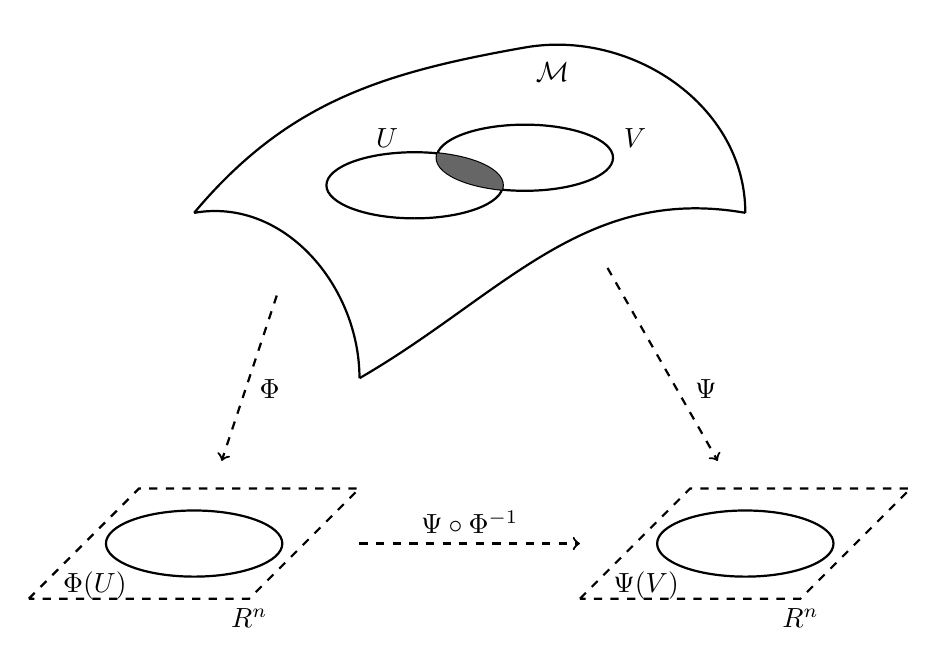
\begin{tikzpicture}[thick,scale=0.7] 
\draw[color=black] (0,0) to [out=50,in=190] (6,3);
\draw[color=black] (6,3) to [out=10,in=90] (10,0);
\draw[color=black] (10,0) to [out=170,in=30] (3,-3);
\draw[color=black] (3,-3) to [out=90,in=10] (0,0);
\filldraw (6.5,2.2) circle (0pt) node[above] {$\Mcal$}; 
\def\firstellipse{(4,0.5) ellipse (1.6 and 0.6)};
\def\secondellipse{(6,1) ellipse (1.6 and 0.6)};
\draw[color=black] \firstellipse \secondellipse;
\filldraw (3.5,1) circle (0pt) node[above] {$U$}; 
\filldraw (8,01) circle (0pt) node[above] {$V$}; 
\begin{scope}
\clip \firstellipse;
\fill[white!40!black] \secondellipse;
\end{scope}
\draw[dashed] (-3,-7) -- (-1,-5) -- (3,-5) -- (1,-7) -- (-3,-7);
\filldraw (1,-7) circle (0pt) node[below] {$\Rbb^n$}; 
\draw[color=black] (0,-6) ellipse (1.6 and 0.6);
\filldraw (-1.8,-7.2) circle (0pt) node[above] {$\Phi(U)$}; 
\draw[dashed] (7,-7) -- (9,-5) -- (13,-5) -- (11,-7) -- (7,-7);
\filldraw (11,-7) circle (0pt) node[below] {$\Rbb^n$}; 
\draw[color=black] (10,-6) ellipse (1.6 and 0.6); 
\filldraw (8.2,-7.2) circle (0pt) node[above] {$\Psi(V)$};
\draw[->,dashed,color=black] (1.5,-1.5) -- (0.5,-4.5);
\filldraw (1,-3.2) circle (0pt) node[right] {$\Phi$}; 
\draw[->,dashed,color=black] (7.5,-1) -- (9.5,-4.5);
\filldraw (8.9,-3.2) circle (0pt) node[right] {$\Psi$}; 
\draw[->,dashed,color=black] (3,-6) -- (7,-6);
\filldraw (5,-6) circle (0pt) node[above] {$\Psi \circ \Phi^{-1}$}; 
\end{tikzpicture}}

\newcommand{\manifoldMaps}{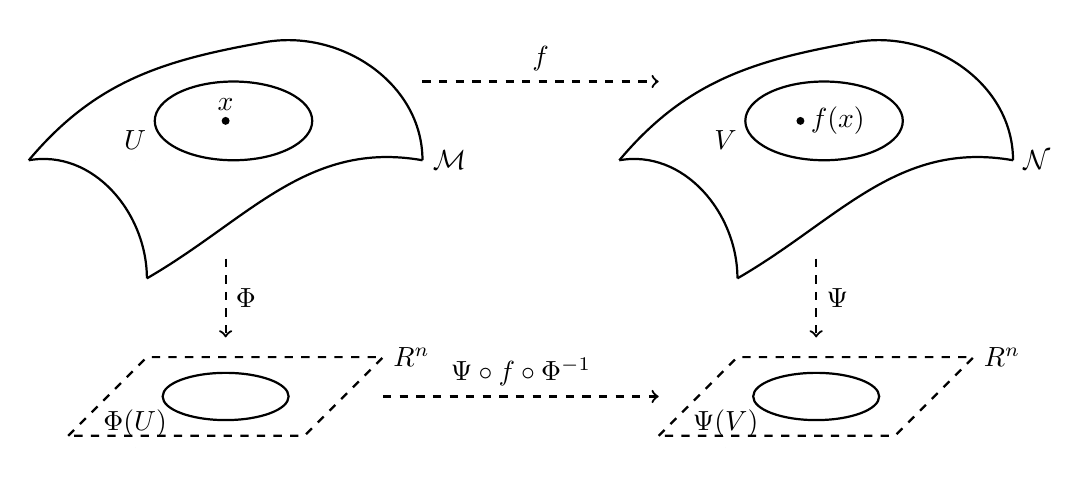
\begin{tikzpicture}[thick,scale=0.5] 
\draw[color=black] (0,0) to [out=50,in=190] (6,3);
\draw[color=black] (6,3) to [out=10,in=90] (10,0);
\draw[color=black] (10,0) to [out=170,in=30] (3,-3);
\draw[color=black] (3,-3) to [out=90,in=10] (0,0);
\draw[color=black] (5.2,1) ellipse (2 and 1);
\filldraw (10,0) circle (0pt) node[right] {$\Mcal$}; 
\filldraw (2.7,0) circle (0pt) node[above] {$U$};
\filldraw (5,1) circle (2pt) node[above] {$x$};
\draw[color=black] (15,0) to [out=50,in=190] (21,3);
\draw[color=black] (21,3) to [out=10,in=90] (25,0);
\draw[color=black] (25,0) to [out=170,in=30] (18,-3);
\draw[color=black] (18,-3) to [out=90,in=10] (15,0);
\draw[color=black] (20.2,1) ellipse (2 and 1);
\filldraw (25,0) circle (0pt) node[right] {$\Ncal$}; 
\filldraw (17.7,0) circle (0pt) node[above] {$V$}; 
\filldraw (19.6,1) circle (2pt) node[right] {$f(x)$};
\draw[->,color=black,dashed] (5,-2.5) -- (5,-4.5);
\filldraw (5,-3.5) circle (0pt) node[right] {$\Phi$}; 
\draw[dashed] (1,-7) -- (3,-5) -- (9,-5) -- (7,-7) -- (1,-7);
\draw[color=black] (5,-6) ellipse (1.6 and 0.6);
\filldraw (9,-5) circle (0pt) node[right] {$\Rbb^n$}; 
\filldraw (2.7,-7.3) circle (0pt) node[above] {$\Phi(U)$}; 
\draw[->,color=black,dashed] (20,-2.5) -- (20,-4.5);
\filldraw (20,-3.5) circle (0pt) node[right] {$\Psi$}; 
\draw[dashed] (16,-7) -- (18,-5) -- (24,-5) -- (22,-7) -- (16,-7);
\draw[color=black] (20,-6) ellipse (1.6 and 0.6);
\filldraw (24,-5) circle (0pt) node[right] {$\Rbb^n$}; 
\filldraw (17.7,-7.3) circle (0pt) node[above] {$\Psi(V)$}; 
\draw[->,color=black,dashed] (9,-6) -- (16,-6);
\filldraw (12.5,-6) circle (0pt) node[above] {$\Psi \circ f \circ \Phi^{-1}$}; 
\draw[->,color=black,dashed] (10,2) -- (16,2);
\filldraw (13,2) circle (0pt) node[above] {$f$}; 
\end{tikzpicture}}

\newcommand{\manifoldFunction}{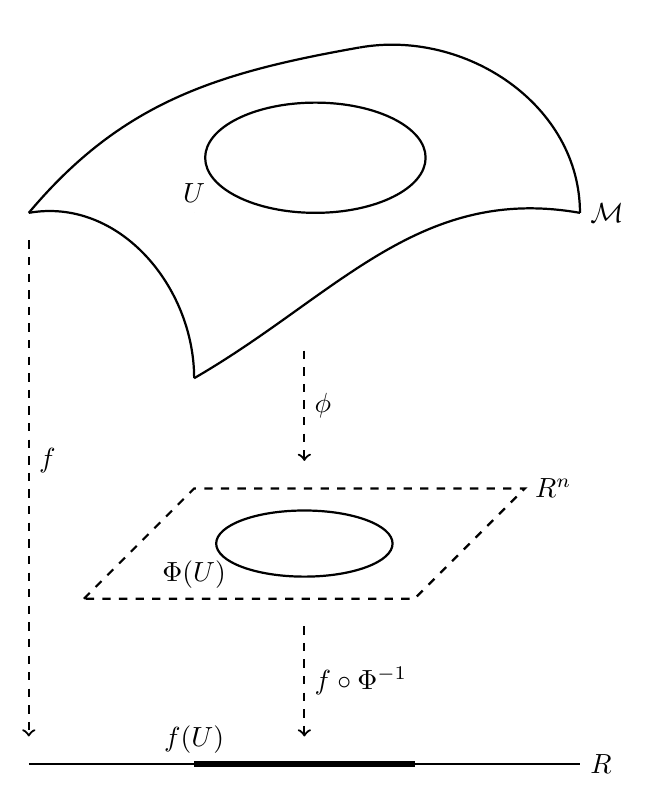
\begin{tikzpicture}[thick,scale=0.7] 
\draw[color=black] (0,0) to [out=50,in=190] (6,3);
\draw[color=black] (6,3) to [out=10,in=90] (10,0);
\draw[color=black] (10,0) to [out=170,in=30] (3,-3);
\draw[color=black] (3,-3) to [out=90,in=10] (0,0);
\draw[color=black] (5.2,1) ellipse (2 and 1);
\filldraw (10,0) circle (0pt) node[right] {$\Mcal$}; 
\filldraw (3,0) circle (0pt) node[above] {$U$}; 
\draw[->,color=black,dashed] (5,-2.5) -- (5,-4.5);
\filldraw (5,-3.5) circle (0pt) node[right] {$\phi$}; 
\draw[dashed] (1,-7) -- (3,-5) -- (9,-5) -- (7,-7) -- (1,-7);
\draw[color=black] (5,-6) ellipse (1.6 and 0.6);
\filldraw (9,-5) circle (0pt) node[right] {$\Rbb^n$}; 
\filldraw (3,-7) circle (0pt) node[above] {$\Phi(U)$}; 
\draw[->,color=black,dashed] (5,-7.5) -- (5,-9.5);
\filldraw (5,-8.5) circle (0pt) node[right] {$f \circ \Phi^{-1}$}; 
\draw[line width=0.8mm,color=black] (3,-10) -- (7,-10);
\draw[color=black] (0,-10) -- (10,-10);
\filldraw (10,-10) circle (0pt) node[right] {$\Rbb$};
\filldraw (3,-10) circle (0pt) node[above] {$f(U)$}; 
\draw[->,color=black,dashed] (0,-0.5) -- (0,-9.5);
\filldraw (0,-4.5) circle (0pt) node[right] {$f$}; 
\end{tikzpicture}}

\newcommand{\tangentSpace}{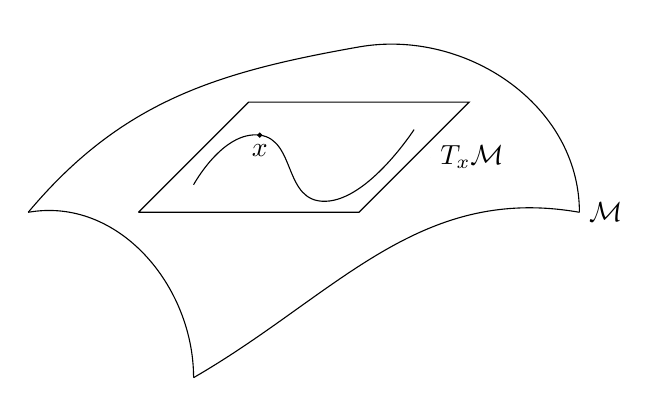
\begin{tikzpicture}[scale=0.7] 
\draw[color=black] (0,0) to [out=50,in=190] (6,3);
\draw[color=black] (6,3) to [out=10,in=90] (10,0);
\draw[color=black] (10,0) to [out=170,in=30] (3,-3);
\draw[color=black] (3,-3) to [out=90,in=10] (0,0);
\filldraw (10,0) circle (0pt) node[right] {$\Mcal$};  
\draw[color=black] (2,0) -- (4,2) -- (8,2) -- (6,0) -- (2,0);
\filldraw (7.3,1) circle (0pt) node[right] {$T_x\Mcal$};
\draw [color=black] plot [smooth,tension=1] coordinates {(3,0.5) (4.2,1.4) (5.4,0.2) (7,1.5)};
\filldraw (4.2,1.4) circle (1pt) node[below] {$x$};
\end{tikzpicture}}

\newcommand{\bundle}{\begin{tikzpicture}[scale=1]
\draw[->,color=black] (0,0) -- (3,0);
\filldraw (1.5,0) circle (0pt) node[above] {$\psi$};
\draw[->,color=black] (0,-0.2) -- (1.3,-1.5);
\filldraw (0.5,-0.8) circle (0pt) node[left] {$\pi$};
\draw[->,color=black] (3,-0.2) -- (1.7,-1.5);
\filldraw (2.5,-0.8) circle (0pt) node[right] {$\psf\rsf_1$};
%
\filldraw (0,0) circle (0pt) node[left] {$\pi^{-1}(U)$};
\filldraw (3,0) circle (0pt) node[right] {$U \times \{ E_x \}$};
\filldraw (1.5,-1.5) circle (0pt) node[below] {$U$};
\end{tikzpicture}}

\newcommand{\expoMap}{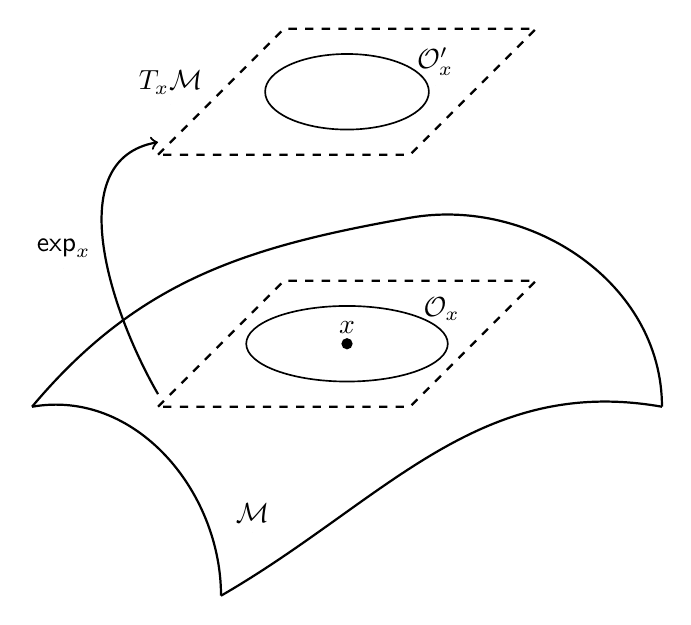
\begin{tikzpicture}[thick,scale=0.8] 
\draw[color=black] (0,0) to [out=50,in=190] (6,3);
\draw[color=black] (6,3) to [out=10,in=90] (10,0);
\draw[color=black] (10,0) to [out=170,in=30] (3,-3);
\draw[color=black] (3,-3) to [out=90,in=10] (0,0);
\draw[semithick] (5,1) ellipse (1.6 and 0.6); 
\draw[dashed] (2,0) -- (4,2) -- (8,2) -- (6,0) -- (2,0);
\draw[color=black,->] (2,0.2) to [out=120,in=190] (2,4.2);
\draw[semithick] (5,5) ellipse (1.3 and 0.6); 
\draw[dashed] (2,4) -- (4,6) -- (8,6) -- (6,4) -- (2,4);
\filldraw (3.5,-2) circle (0pt) node[above] {$\Mcal$}; 
\filldraw (5,1) circle (2pt) node[above] {$x$};
\filldraw (6.5,1.2) circle (0pt) node[above] {$\Ocal_x$};
\filldraw (6.4,5.1) circle (0pt) node[above] {$\Ocal^\prime_x$};
\filldraw (2.2,4.8) circle (0pt) node[above] {$T_x\Mcal$};
\filldraw (0.5,2.2) circle (0pt) node[above] {$\mathsf{exp}_x$};
\end{tikzpicture}}

\newcommand{\geodesic}{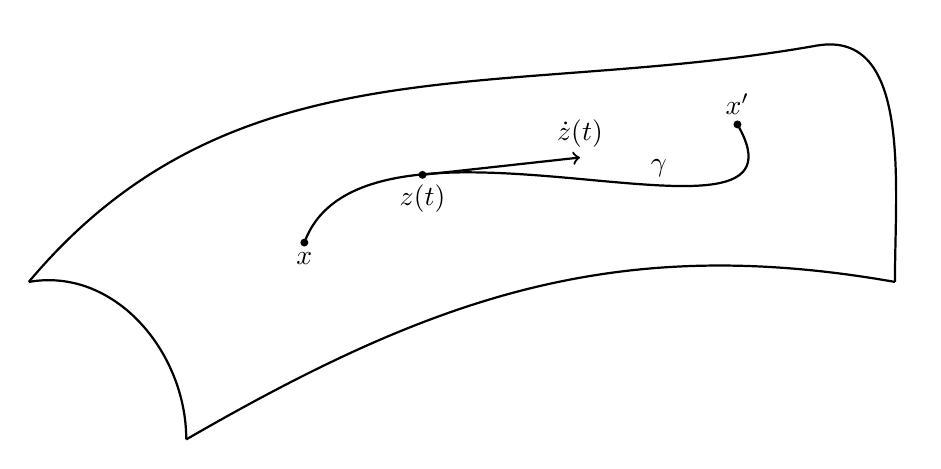
\begin{tikzpicture}[thick,scale=1] 
\draw[color=black] (-2,-1) to [out=50,in=190] (8,2);
\draw[color=black] (8,2) to [out=10,in=90] (9,-1);
\draw[color=black] (9,-1) to [out=170,in=30] (0,-3);
\draw[color=black] (0,-3) to [out=90,in=10] (-2,-1); 
\draw[color=black] (1.5,-0.5) to [out=70,in=-60] (7,1);
\filldraw (1.5,-0.5) circle (1pt) node[below] {$x$};
\filldraw (7,1) circle (1pt) node[above] {$x^\prime$}; 
\filldraw (3,0.36) circle (1pt) node[below] {$z(t)$};
\draw[->] (3,0.36) -- (5,0.58) node[above] {$\dot{z}(t)$};
\filldraw (6,0.2) circle (0pt) node[above] {$\gamma$};
\end{tikzpicture}}

\newcommand{\lightcone}{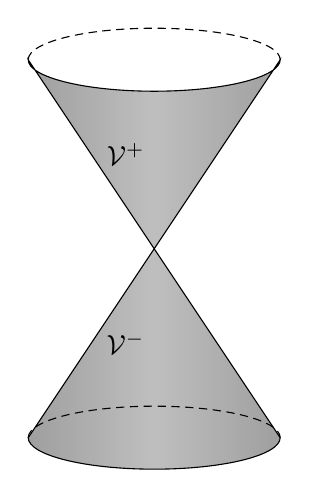
\begin{tikzpicture}[scale=0.8]
\fill[left color=gray!50!black,right color=gray!50!black,middle color=gray!50,shading=axis,opacity=0.25] (2,6) -- (0,3) -- (-2,6) arc (180:360:2cm and 0.5cm);
\draw (-2,6) arc (180:360:2cm and 0.5cm) -- (0,3) -- cycle;
\draw[densely dashed] (-2,6) arc (180:0:2cm and 0.5cm);
\fill[left color=gray!50!black,right color=gray!50!black,middle color=gray!50,shading=axis,opacity=0.25] (2,0) -- (0,3) -- (-2,0) arc (180:360:2cm and 0.5cm);
\draw (-2,0) arc (180:360:2cm and 0.5cm) -- (0,3) -- cycle;
\draw[densely dashed] (-2,0) arc (180:0:2cm and 0.5cm);
\filldraw[black] (0,1.5) circle (0pt) node[left] {$\Vcal^{-}$};
\filldraw[black] (0,4.5) circle (0pt) node[left] {$\Vcal^{+}$};
\end{tikzpicture}}

\newcommand{\supportPropagator}{
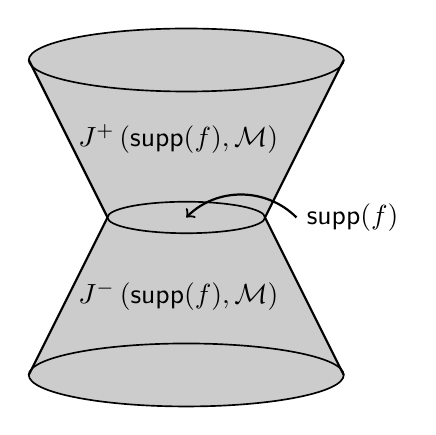
\begin{tikzpicture}[thick,scale=1]
\fill[color=white!80!black] (0,2) ellipse (2 and 0.4);
\fill[color=white!80!black] (0,0) ellipse (1 and 0.2);
\fill[color=white!80!black] (0,-2) ellipse (2 and 0.4);
\fill[color=white!80!black] (2, 2) -- (1, 0) -- (-1,0) -- (-2,2) -- (2,2);
\fill[color=white!80!black] (2, -2) -- (1, 0) -- (-1,0) -- (-2,-2) -- (2,-2);
\draw[semithick] (0,2) ellipse (2 and 0.4);
\draw (2,2) -- (1,0);
\draw (-2,2) -- (-1,0);
\draw[semithick] (0,0) ellipse (1 and 0.2);
\draw (-2,-2) -- (-1,0);
\draw (2,-2) -- (1,0);
\draw[semithick] (0,-2) ellipse (2 and 0.4);
\filldraw[black] (-1.5,1) circle (0pt) node[right] {$J^+\left(\supp(f),\Mcal\right)$};
\filldraw[black] (1.4,0) circle (0pt) node[right] {$\supp(f)$};
\filldraw[black] (-1.5,-1) circle (0pt) node[right] {$J^-\left(\supp(f),\Mcal\right)$};
\draw[->] (1.4,0) to [bend right=45] (0,0);
\end{tikzpicture}}

\newcommand{\DeltaF}{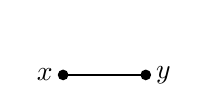
\begin{tikzpicture}[thick,scale=1.5]
\useasboundingbox (-0.3,-0.07) rectangle (1,0.4);
\filldraw (0,0) circle (1pt) node[left] {$x$};
\filldraw (0.7,0) circle (1pt) node[right] {$y$};
\draw (0,0) -- (0.7,0);
\end{tikzpicture} }

\newcommand{\DeltaPM}{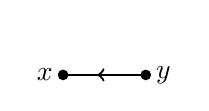
\begin{tikzpicture}[thick,scale=1.5]
\useasboundingbox (-0.3,-0.07) rectangle (1,0.4);
\filldraw (0,0) circle (1pt) node[left] {$x$};
\filldraw (0.7,0) circle (1pt) node[right] {$y$};
\draw[GFleche] (0,0) -- (0.7,0);
\end{tikzpicture} }

\newcommand{\DeltaR}{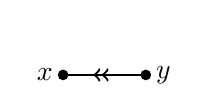
\begin{tikzpicture}[thick,scale=1.5]
\useasboundingbox (-0.3,-0.07) rectangle (1,0.4);
\filldraw (0,0) circle (1pt) node[left] {$x$};
\filldraw (0.7,0) circle (1pt) node[right] {$y$};
\draw[GDoubleFleche] (0,0) -- (0.7,0);
\end{tikzpicture} }

\newcommand{\LineCross}{\begin{tikzpicture}[thick,scale=1.5]
\useasboundingbox (-0.3,-0.07) rectangle (1,0.4);
\draw (0,0) -- (0.7,0);
\filldraw (0.35,0) node[cross] {};
\end{tikzpicture} }

\newcommand{\CrossEdges}{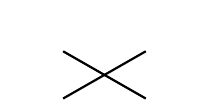
\begin{tikzpicture}[thick,scale=1.5]
\useasboundingbox (-0.3,-0.07) rectangle (1,0.4);
\draw (0,-0.2) -- (0.7,0.2);
\draw (0,0.2) -- (0.7,-0.2);
\end{tikzpicture} }

\newcommand{\Uno}{\begin{tikzpicture}[thick,scale=1.5]
\useasboundingbox (-0.3,-0.07) rectangle (1.5,0.8);
\draw[GFleche] (0,0) -- (0.5,0);
\filldraw (0,0) circle (1pt) node[left] {$x$};
\filldraw (0.5,0) circle (1pt) node[right] {$y$};
\end{tikzpicture} }

\newcommand{\Due}{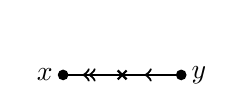
\begin{tikzpicture}[thick,scale=1.5]
\useasboundingbox (-0.3,-0.07) rectangle (1.3,0.4);
\draw[GDoubleFleche] (0,0) -- (0.5,0);
\draw[GFleche] (0.5,0) -- (1,0);
\filldraw (0,0) circle (1pt) node[left] {$x$};
\filldraw (0.5,0) node[cross] {};
\filldraw (1,0) circle (1pt) node[right] {$y$};
\end{tikzpicture} }

\newcommand{\Tre}{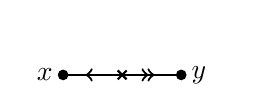
\begin{tikzpicture}[thick,scale=1.5]
\useasboundingbox (-0.3,-0.07) rectangle (1.5,0.4);
\draw[GFleche] (0,0) -- (0.5,0);
\draw[DDoubleFleche] (0.5,0) -- (1,0);
\filldraw (0,0) circle (1pt) node[left] {$x$};
\filldraw (0.5,0) node[cross] {};
\filldraw (1,0) circle (1pt) node[right] {$y$};
\end{tikzpicture} }

\newcommand{\Quattro}{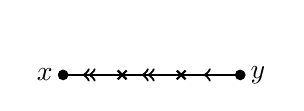
\begin{tikzpicture}[thick,scale=1.5]
\useasboundingbox (-0.3,-0.07) rectangle (1.8,0.4);
\draw[GDoubleFleche] (0,0) -- (0.5,0);
\draw[GDoubleFleche] (0.5,0) -- (1,0);
\draw[GFleche] (1,0) -- (1.5,0);
\filldraw (0,0) circle (1pt) node[left] {$x$};
\filldraw (0.5,0) node[cross] {};
\filldraw (1,0) node[cross] {};
\filldraw (1.5,0) circle (1pt) node[right] {$y$};
\end{tikzpicture} }

\newcommand{\Cinque}{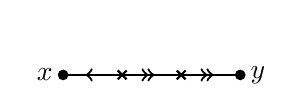
\begin{tikzpicture}[thick,scale=1.5]
\useasboundingbox (-0.3,-0.07) rectangle (1.8,0.4);
\draw[GFleche] (0,0) -- (0.5,0);
\draw[DDoubleFleche] (0.5,0) -- (1,0);
\draw[DDoubleFleche] (1,0) -- (1.5,0);
\filldraw (0,0) circle (1pt) node[left] {$x$};
\filldraw (0.5,0) node[cross] {};
\filldraw (1,0) node[cross] {};
\filldraw (1.5,0) circle (1pt) node[right] {$y$};
\end{tikzpicture} }

\newcommand{\Sei}{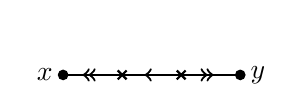
\begin{tikzpicture}[thick,scale=1.5]
\useasboundingbox (-0.3,-0.07) rectangle (1.8,0.4);
\draw[GDoubleFleche] (0,0) -- (0.5,0);
\draw[GFleche] (0.5,0) -- (1,0);
\draw[DDoubleFleche] (1,0) -- (1.5,0);
\filldraw (0,0) circle (1pt) node[left] {$x$};
\filldraw (0.5,0) node[cross] {};
\filldraw (1,0) node[cross] {};
\filldraw (1.5,0) circle (1pt) node[right] {$y$};
\end{tikzpicture} }

\newcommand{\Sette}{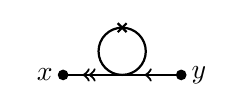
\begin{tikzpicture}[thick,scale=1.5]
\useasboundingbox (-0.3,-0.07) rectangle (1.3,0.4);
\draw[GDoubleFleche] (0,0) -- (0.5,0);
\draw[GFleche] (0.5,0) -- (1,0);
\draw (0.5,0.2) circle (0.2cm);
\filldraw (0,0) circle (1pt) node[left] {$x$};
\filldraw (0.5,0.4) node[cross] {};
\filldraw (1,0) circle (1pt) node[right] {$y$};
\end{tikzpicture} }

\newcommand{\Otto}{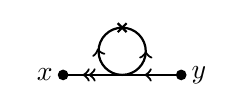
\begin{tikzpicture}[thick,scale=1.5]
\useasboundingbox (-0.3,-0.07) rectangle (1.3,0.4);
\draw[GDoubleFleche] (0,0) -- (0.5,0);
\draw[GFleche] (0.5,0) -- (1,0);
\draw[CFleche] (0.5,0.2) circle (0.2cm);
\filldraw (0,0) circle (1pt) node[left] {$x$};
\filldraw (0.5,0.4) node[cross] {};
\filldraw (1,0) circle (1pt) node[right] {$y$};
\end{tikzpicture} }

\newcommand{\Nove}{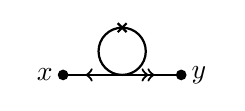
\begin{tikzpicture}[thick,scale=1.5]
\useasboundingbox (-0.3,-0.07) rectangle (1.3,0.4);
\draw[GFleche] (0,0) -- (0.5,0);
\draw[DDoubleFleche] (0.5,0) -- (1,0);
\draw (0.5,0.2) circle (0.2cm);
\filldraw (0,0) circle (1pt) node[left] {$x$};
\filldraw (0.5,0.4) node[cross] {};
\filldraw (1,0) circle (1pt) node[right] {$y$};
\end{tikzpicture} }

\newcommand{\Diece}{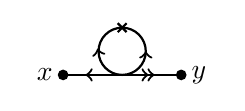
\begin{tikzpicture}[thick,scale=1.5]
\useasboundingbox (-0.3,-0.07) rectangle (1.3,0.4);
\draw[GFleche] (0,0) -- (0.5,0);
\draw[DDoubleFleche] (0.5,0) -- (1,0);
\draw[CFleche] (0.5,0.2) circle (0.2cm);
\filldraw (0,0) circle (1pt) node[left] {$x$};
\filldraw (0.5,0.4) node[cross] {};
\filldraw (1,0) circle (1pt) node[right] {$y$};
\end{tikzpicture} }

\newcommand{\Undici}{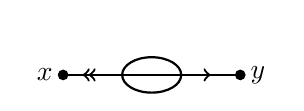
\begin{tikzpicture}[thick,scale=1.5]
\useasboundingbox (-0.3,-0.07) rectangle (1.8,0.4);
\draw[GDoubleFleche] (0,0) -- (0.5,0);
\draw (0.5,0) -- (1,0);
\draw[DFleche] (1,0) -- (1.5,0);
\draw (0.75,0) ellipse (0.25cm and 0.15cm);
\filldraw (0,0) circle (1pt) node[left] {$x$};
\filldraw (1.5,0) circle (1pt) node[right] {$y$};
\end{tikzpicture} }

\newcommand{\Dodici}{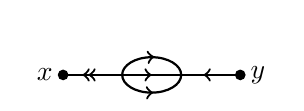
\begin{tikzpicture}[thick,scale=1.5]
\useasboundingbox (-0.3,-0.07) rectangle (1.8,0.4);
\draw[GDoubleFleche] (0,0) -- (0.5,0);
\draw[DFleche] (0.5,0) -- (1,0);
\draw[GFleche] (1,0) -- (1.5,0);
\draw[EDleche] (0.75,0) ellipse (0.25cm and 0.15cm);
\filldraw (0,0) circle (1pt) node[left] {$x$};
\filldraw (1.5,0) circle (1pt) node[right] {$y$};
\end{tikzpicture} }

\newcommand{\Tredici}{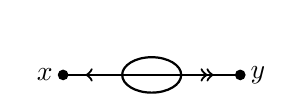
\begin{tikzpicture}[thick,scale=1.5]
\useasboundingbox (-0.3,-0.07) rectangle (1.8,0.4);
\draw[GFleche] (0,0) -- (0.5,0);
\draw (0.5,0) -- (1,0);
\draw[DDoubleFleche] (1,0) -- (1.5,0);
\draw (0.75,0) ellipse (0.25cm and 0.15cm);
\filldraw (0,0) circle (1pt) node[left] {$x$};
\filldraw (1.5,0) circle (1pt) node[right] {$y$};
\end{tikzpicture} }

\newcommand{\Quattrodici}{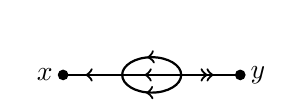
\begin{tikzpicture}[thick,scale=1.5]
\useasboundingbox (-0.3,-0.07) rectangle (1.8,0.4);
\draw[GFleche] (0,0) -- (0.5,0);
\draw[GFleche] (0.5,0) -- (1,0);
\draw[DDoubleFleche] (1,0) -- (1.5,0);
\draw[EGleche] (0.75,0) ellipse (0.25cm and 0.15cm);
\filldraw (0,0) circle (1pt) node[left] {$x$};
\filldraw (1.5,0) circle (1pt) node[right] {$y$};
\end{tikzpicture} }

\newcommand{\Quindici}{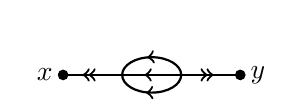
\begin{tikzpicture}[thick,scale=1.5]
\useasboundingbox (-0.3,-0.07) rectangle (1.8,0.4);
\draw[GDoubleFleche] (0,0) -- (0.5,0);
\draw[GFleche] (0.5,0) -- (1,0);
\draw[DDoubleFleche] (1,0) -- (1.5,0);
\draw[EGleche] (0.75,0) ellipse (0.25cm and 0.15cm);
\filldraw (0,0) circle (1pt) node[left] {$x$};
\filldraw (1.5,0) circle (1pt) node[right] {$y$};
\end{tikzpicture} }

\newcommand{\FG}{
\begin{tikzpicture}[thick,scale=1.5]
\useasboundingbox (-0.1,-0.07) rectangle (0.5,0.4);
\filldraw (0,0) circle (1.3pt);
\filldraw (0.4,0) circle (1.3pt);
\end{tikzpicture} }

\newcommand{\FoneG}{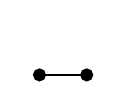
\begin{tikzpicture}[thick,scale=1.5]
\useasboundingbox (-0.1,-0.07) rectangle (0.5,0.4);
\filldraw (0,0) circle (1.3pt);
\filldraw (0.4,0) circle (1.3pt);
\draw (0,0) -- (0.4,0);
\end{tikzpicture} }

\newcommand{\FtwoG}{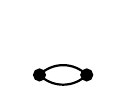
\begin{tikzpicture}[thick,scale=1.5]
\useasboundingbox (-0.1,-0.07) rectangle (0.5,0.4);
\filldraw (0,0) circle (1.3pt);
\filldraw (0.4,0) circle (1.3pt);
\draw (0,0) edge [out=45,in=135] node[above] {} (0.4,0);
\draw (0,0) edge [out=-45,in=-135] node[above] {} (0.4,0);
\end{tikzpicture} }

\newcommand{\FthreeG}{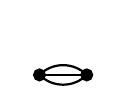
\begin{tikzpicture}[thick,scale=1.5]
\useasboundingbox (-0.1,-0.07) rectangle (0.5,0.4);
\filldraw (0,0) circle (1.3pt);
\filldraw (0.4,0) circle (1.3pt);
\draw (0,0) edge [out=45,in=135] node[above] {} (0.4,0);
\draw (0,0) -- (0.4,0);
\draw (0,0) edge [out=-45,in=-135] node[above] {} (0.4,0);
\end{tikzpicture} }

\newcommand{\FnG}{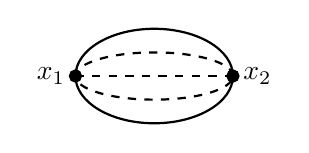
\begin{tikzpicture}[thick,scale=1] 
\draw[dashed] (0,0) circle (1cm and 0.3cm);
\draw (0,0) circle (1cm and 0.6cm);
\draw[dashed] (-1,0) -- (1,0);
\filldraw (-1,0) circle (2pt) node[left] {$x_1$};
\filldraw (1,0) circle (2pt) node[right] {$x_2$};
\end{tikzpicture}}

\newcommand{\FGH}{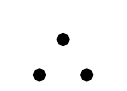
\begin{tikzpicture}[thick,scale=1.5]
\useasboundingbox (-0.1,0.1) rectangle (0.5,0.4);
\filldraw (0,0) circle (1.3pt);
\filldraw (0.4,0) circle (1.3pt);
\filldraw (0.2,0.3) circle (1.3pt);
\end{tikzpicture} }

\newcommand{\FoneGHF}{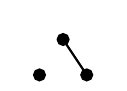
\begin{tikzpicture}[thick,scale=1.5]
\useasboundingbox (-0.1,0.1) rectangle (0.5,0.4);
\filldraw (0,0) circle (1.3pt);
\filldraw (0.4,0) circle (1.3pt);
\filldraw (0.2,0.3) circle (1.3pt);
\draw (0.2,0.3) -- (0.4,0);
\end{tikzpicture} }

\newcommand{\FGoneHF}{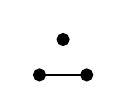
\begin{tikzpicture}[thick,scale=1.5]
\useasboundingbox (-0.1,0.1) rectangle (0.5,0.4);
\filldraw (0,0) circle (1.3pt);
\filldraw (0.4,0) circle (1.3pt);
\filldraw (0.2,0.3) circle (1.3pt);
\draw (0,0) -- (0.4,0);
\end{tikzpicture} }

\newcommand{\FGHoneF}{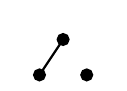
\begin{tikzpicture}[thick,scale=1.5]
\useasboundingbox (-0.1,0.1) rectangle (0.5,0.4);
\filldraw (0,0) circle (1.3pt);
\filldraw (0.4,0) circle (1.3pt);
\filldraw (0.2,0.3) circle (1.3pt);
\draw (0,0) -- (0.2,0.3);
\end{tikzpicture} }

\newcommand{\FoneGoneHF}{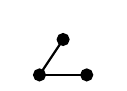
\begin{tikzpicture}[thick,scale=1.5]
\useasboundingbox (-0.1,0.1) rectangle (0.5,0.4);
\filldraw (0,0) circle (1.3pt);
\filldraw (0.4,0) circle (1.3pt);
\filldraw (0.2,0.3) circle (1.3pt);
\draw (0,0) -- (0.2,0.3);
\draw (0.4,0) -- (0,0);
\end{tikzpicture} }

\newcommand{\FoneGHoneF}{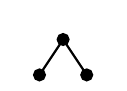
\begin{tikzpicture}[thick,scale=1.5]
\useasboundingbox (-0.1,0.1) rectangle (0.5,0.4);
\filldraw (0,0) circle (1.3pt);
\filldraw (0.4,0) circle (1.3pt);
\filldraw (0.2,0.3) circle (1.3pt);
\draw (0,0) -- (0.2,0.3);
\draw (0.4,0) -- (0.2,0.3);
\end{tikzpicture} }

\newcommand{\FGoneHoneF}{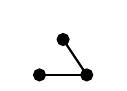
\begin{tikzpicture}[thick,scale=1.5]
\useasboundingbox (-0.1,0.1) rectangle (0.5,0.4);
\filldraw (0,0) circle (1.3pt);
\filldraw (0.4,0) circle (1.3pt);
\filldraw (0.2,0.3) circle (1.3pt);
\draw (0.4,0) -- (0.2,0.3);
\draw (0.4,0) -- (0,0);
\end{tikzpicture} }

\newcommand{\FtwoGHF}{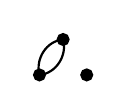
\begin{tikzpicture}[thick,scale=1.5]
\useasboundingbox (-0.1,0.1) rectangle (0.5,0.4);
\filldraw (0,0) circle (1.3pt);
\filldraw (0.4,0) circle (1.3pt);
\filldraw (0.2,0.3) circle (1.3pt);
\draw (0,0) edge [out=105,in=185] node[above] {} (0.2,0.3);
\draw (0,0) edge [out=5,in=-75] node[above] {} (0.2,0.3);
\end{tikzpicture} }

\newcommand{\FGtwoHF}{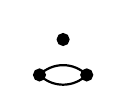
\begin{tikzpicture}[thick,scale=1.5]
\useasboundingbox (-0.1,0.1) rectangle (0.5,0.4);
\filldraw (0,0) circle (1.3pt);
\filldraw (0.4,0) circle (1.3pt);
\filldraw (0.2,0.3) circle (1.3pt);
\draw (0,0) edge [out=45,in=135] node[above] {} (0.4,0);
\draw (0,0) edge [out=-45,in=-135] node[above] {} (0.4,0);
\end{tikzpicture} }

\newcommand{\FGHtwoF}{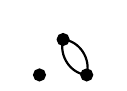
\begin{tikzpicture}[thick,scale=1.5]
\useasboundingbox (-0.1,0.1) rectangle (0.5,0.4);
\filldraw (0,0) circle (1.3pt);
\filldraw (0.4,0) circle (1.3pt);
\filldraw (0.2,0.3) circle (1.3pt);
\draw (0.4,0) edge [out=75,in=-5] node[above] {} (0.2,0.3);
\draw (0.4,0) edge [out=-185,in=-105] node[above] {} (0.2,0.3);
\end{tikzpicture} }

\newcommand{\FtwoGoneHoneF}{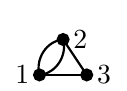
\begin{tikzpicture}[thick,scale=1.5]
\useasboundingbox (-0.1,0.1) rectangle (0.5,0.4);
\filldraw (0,0) circle (1.3pt) node[left] {$1$};
\filldraw (0.4,0) circle (1.3pt) node[right] {$3$};
\filldraw (0.2,0.3) circle (1.3pt) node[right] {$2$};
\draw (0,0) edge [out=105,in=185] node[above] {} (0.2,0.3);
\draw (0,0) edge [out=5,in=-75] node[above] {} (0.2,0.3);
\draw (0.4,0) -- (0.2,0.3);
\draw (0.4,0) -- (0,0);
\end{tikzpicture} }

\newcommand{\FtwoGtwoHoneF}{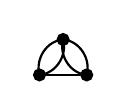
\begin{tikzpicture}[thick,scale=1.5]
\useasboundingbox (-0.1,0.1) rectangle (0.5,0.4);
\filldraw (0,0) circle (1.3pt);
\filldraw (0.4,0) circle (1.3pt);
\filldraw (0.2,0.3) circle (1.3pt);
\draw (0,0) edge [out=105,in=185] node[above] {} (0.2,0.3);
\draw (0,0) edge [out=5,in=-75] node[above] {} (0.2,0.3);
\draw (0.4,0) edge [out=75,in=-5] node[above] {} (0.2,0.3);
\draw (0.4,0) edge [out=-185,in=-105] node[above] {} (0.2,0.3);
\draw (0.4,0) -- (0,0);
\end{tikzpicture} }

\newcommand{\FnGnHnF}{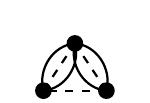
\begin{tikzpicture}[thick,scale=2]
\useasboundingbox (-0.1,0.1) rectangle (0.5,0.4);
\filldraw (0,0) circle (1.3pt);
\filldraw (0.4,0) circle (1.3pt);
\filldraw (0.2,0.3) circle (1.3pt);
\draw (0,0) edge [out=105,in=185] node[above] {} (0.2,0.3);
\draw (0,0) edge [out=5,in=-75] node[above] {} (0.2,0.3);
\draw (0.4,0) edge [out=75,in=-5] node[above] {} (0.2,0.3);
\draw (0.4,0) edge [out=-185,in=-105] node[above] {} (0.2,0.3);
\draw[dashed] (0,0) -- (0.2,0.3);
\draw[dashed] (0.4,0) -- (0.2,0.3);
\draw[dashed] (0.4,0) -- (0,0);
\end{tikzpicture} }

\newcommand{\catseye}{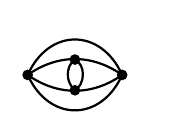
\begin{tikzpicture}[thick,scale=1.5]
\useasboundingbox (0,-0.1) rectangle (1,0.4);
\filldraw (0,0) circle (1pt);
\filldraw (0.4,0.13) circle (1pt);
\filldraw (0.4,-0.13) circle (1pt);
\filldraw (0.8,0) circle (1pt);
\draw (0,0) .. controls (0.18,0.4) and (0.62,0.4) .. (0.8,0);
\draw (0,0) .. controls (0.18,-0.4) and (0.62,-0.4) .. (0.8,0);
\draw (0,0) edge [out=35,in=145] node[above] {} (0.8,0);
\draw (0,0) edge [out=-35,in=-145] node[above] {} (0.8,0);
\draw (0.4,0.13) edge [out=-25,in=30] node[above] {} (0.4,-0.13);
\draw (0.4,0.13) edge [out=-145,in=140] node[above] {} (0.4,-0.13);
\end{tikzpicture} }

\newcommand{\analytic}{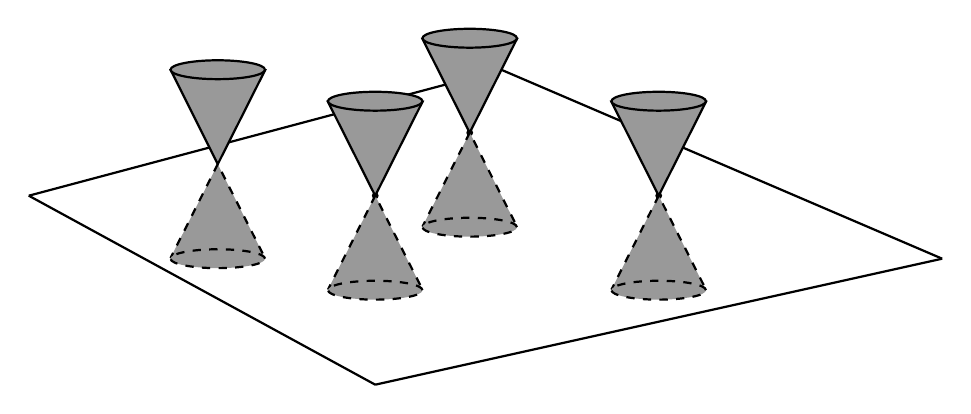
\begin{tikzpicture}[thick,scale=0.4] 
\draw[color=black] (-7,-1) -- (8,3);
\draw[color=black] (8,3) -- (22,-3);
\draw[color=black] (22,-3) -- (4,-7);
\draw[color=black] (4,-7) -- (-7,-1);
\filldraw[color=black] (7,1) circle (2pt);
\draw [fill=black!40!white,opacity=1] (5.5,3.98) -- (8.5,3.98) -- (7,1) -- cycle;
\draw [fill=black!40!white,opacity=1] (7,4) circle (1.5cm and 0.3cm);
\draw [fill=black!40!white,opacity=1,dashed] (5.5,-1.98) -- (8.5,-1.98) -- (7,1) -- cycle;
\draw [fill=black!40!white,opacity=1,dashed] (7,-2) circle (1.5cm and 0.3cm);
\filldraw (4,-1) circle (2pt);
\draw [fill=black!40!white,opacity=1] (2.5,1.98) -- (5.5,1.98) -- (4,-1) -- cycle;
\draw [fill=black!40!white,opacity=1] (4,2) circle (1.5cm and 0.3cm);
\draw [fill=black!40!white,opacity=1,dashed] (2.5,-3.98) -- (5.5,-3.98) -- (4,-1) -- cycle;
\draw [fill=black!40!white,opacity=1,dashed] (4,-4) circle (1.5cm and 0.3cm);
\filldraw (13,-1) circle (2pt);
\draw [fill=black!40!white,opacity=1] (11.5,1.98) -- (14.5,1.98) -- (13,-1) -- cycle;
\draw [fill=black!40!white,opacity=1] (13,2) circle (1.5cm and 0.3cm);
\draw [fill=black!40!white,opacity=1,dashed] (11.5,-3.98) -- (14.5,-3.98) -- (13,-1) -- cycle;
\draw [fill=black!40!white,opacity=1,dashed] (13,-4) circle (1.5cm and 0.3cm);
\draw [fill=black!40!white,opacity=1] (-2.49,2.98) -- (0.5,2.98) -- (-1,0) -- cycle;
\draw [fill=black!40!white,opacity=1] (-1,3) circle (1.5cm and 0.3cm);
\draw [fill=black!40!white,opacity=1,dashed] (-2.5,-2.98) -- (0.5,-2.98) -- (-1,0) -- cycle;
\draw [fill=black!40!white,opacity=1,dashed] (-1,-3) circle (1.5cm and 0.3cm);
\end{tikzpicture}}

\newcommand{\BigFtwoGoneHoneF}{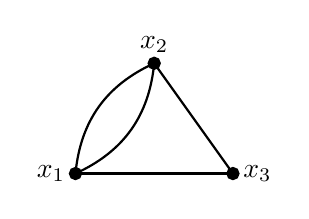
\begin{tikzpicture}[thick,scale=1] 
\draw (0,0) -- (2,0);
\draw (2,0) -- (1,1.4);
\draw [bend left] (0,0) edge (1,1.4);
\draw [bend left] (1,1.4) edge (0,0);
\filldraw (0,0) circle (2pt) node[left] {$x_1$};
\filldraw (2,0) circle (2pt) node[right] {$x_3$};
\filldraw (1,1.4) circle (2pt) node[above] {$x_2$};
\end{tikzpicture}}

%----------------------------------------------------------------------------%

\title{Analytic regularization of quantum field theories on curved backgrounds}

\author{Antoine Géré}

\date{February 24th, 2016}

\institute{Università degli studi di Genova}

\conference{Dipartimento di Matematica}

\shortconference{\href{http://www.th.u-psud.fr/}{LPT Orsay}}

%============================================================================%
\begin{document}
%============================================================================%

\selectlanguage{english}

%----------------------------------------------------------------------------%

{% 
\setbeamertemplate{footline}{} 
\setbeamertemplate{headline}{}
\setbeamertemplate{background}{
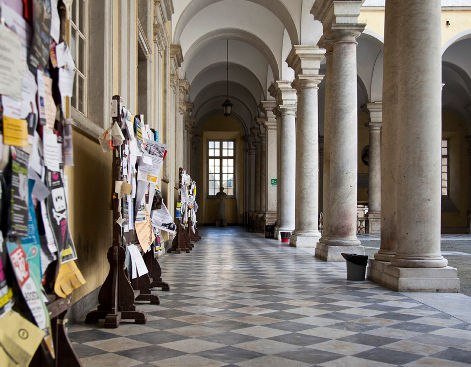
\includegraphics[width=\paperwidth,height=\paperheight]{./presentation.jpg}
}
\begin{frame}[plain]
\titlepage
\end{frame}
}%


%----------------------------------------------------------------------------%

\begin{frame}
 
\frametitle{Interacting quantum field theory -- a brief presentation}

\vfill

\begin{itemize}

\item rigorous study of \textbf{Quantum Field Theory}\\
$\to$ \ \textbf{scalar field} $\phi$

\item \textbf{Interacting theory}
%
\vspace*{-5pt}
\begin{equation*} 
\Psf \phi + \Vsf^{(1)}(\phi) = \left( \Box + \xi R + m^2 \right) \phi + \Vsf^{(1)}(\phi)  = 0
\vspace*{-5pt}
\end{equation*}
%
$\to$ \ local / non linear potential, e.g : $\Vsf(\phi) = \mathop{\mathlarger{\int_{\Mcal}}} \dsf x \ \mathop{\mathlarger{\frac{\lambda}{4!}}} \ f(x) \ \phi(x)^4$ \\[4pt]

$\to$ \ \textbf{perturbative theory} : (expansion in series w.r.t. coupling constant $\lambda$) \\[6pt]

\textbf{Problems occuring} : \par

\vspace*{-12pt}
\begin{block}{\vspace*{-3ex}}
\vspace*{-5pt}\hspace*{12pt}%
\textbf{1.} ultraviolet (UV) divergences occurring at very high energy
\end{block}
\vspace*{-5pt}
\textbf{2.} infrared (IR) divergences occurring at very low energy

\textbf{3.} and the series usually do not converge in any rigorous way

\end{itemize}

\vfill

\end{frame}

%----------------------------------------------------------------------------%

\begin{frame}

\frametitle{Publications}

\begin{exampleblock}{\vspace*{-3ex}}
\vspace*{-5pt}

\paper{%
A. Géré, P. Vitale, and J.-C. Wallet}{%
Quantum gauge theories on noncommutative 3-d space}{%
1312.6145 [hep-th]}{%
http://arxiv.org/abs/1312.6145}{%
Physical Review D 90 (2014) 045019}{%
10.1103/PhysRevD.90.045019}\par%

\paper{%
A. Géré, and J.-C. Wallet}{%
Spectral theorem in noncommutative field theories: Jacobi dynamics}{%
1402.6976 [math-ph]}{%
http://arxiv.org/abs/1402.6976}{%
J. Phys. Conf. Ser. 634 (2014) 012006}{%
10.1088/1742-6596/634/1/012006}\par%

\paper{%
A. Géré, T. Jurić, and J.-C. Wallet}{%
Noncommutative gauge theories on $\mathbb{R}^3_\lambda$: Perturbatively finite models}{%
1507.08086 [hep-th]}{%
http://arxiv.org/abs/1507.08086}{%
JHEP, 12 (2015) 1--29}{%
10.1007/JHEP12(2015)045}\par%

\end{exampleblock}

\begin{block}{\vspace*{-3ex}}
\vspace*{-5pt}

\paper{%
A. Géré, T.-P. Hack, and N. Pinamonti}{%
An analytic Regularization scheme on curved spacetimes with applications to cosmological spacetimes}{%
1505.00286 [math-ph]}{%
http://arxiv.org/abs/1505.00286}{%
accepted in Classical and Quantum Gravity}{%
http://iopscience.iop.org/0264-9381/}%

\end{block}

\end{frame}

%----------------------------------------------------------------------------%

\begin{frame}

\frametitle{Story \& plan}

\begin{exampleblock}{Motivation}
%
\begin{itemize}
\vspace*{-8pt}    
\item perturbative algebraic quantum field theory (pAQFT) \\
\vspace*{-2pt}
$\to$ \textbf{conceptually well known} \\
\vspace*{-2pt}
\citebeam{Brunetti, Dütsch, Fredenhagen, Hollands, K\"ohler, Rejzner, Wald, ...} \\

\vspace*{-8pt}
\item in pAQFT on curved spacetime (CST) \\
$\to$ procedure \textbf{unconvenient for computations} \\
\vspace*{-2pt}
\citebeam{Brunetti \& Fredenhagen, Hollands \& Wald, Dang} \\
    
\vspace*{-8pt}    
\item desire to use framework of pAQFT for \textbf{cosmological model} ! 
\vspace*{-2pt}  
\end{itemize}
%
\end{exampleblock}

\vfill

\begin{exampleblock}{What I am going to talk about}
\begin{itemize}
\vspace*{-8pt}   
\item \textbf{pAQFT} $\to$ in order to identify the regularization problem! \\

\vspace*{-8pt}
\item a framework for an \textbf{analytic regularization} on CST \\

\vspace*{-8pt}
\item \textbf{explicit computations} on a particular cosmological spacetime

\end{itemize}
\end{exampleblock}
%
\end{frame}

%----------------------------------------------------------------------------%

{%
\setbeamertemplate{footline}{} 
\setbeamertemplate{headline}{}
\setbeamertemplate{background}{
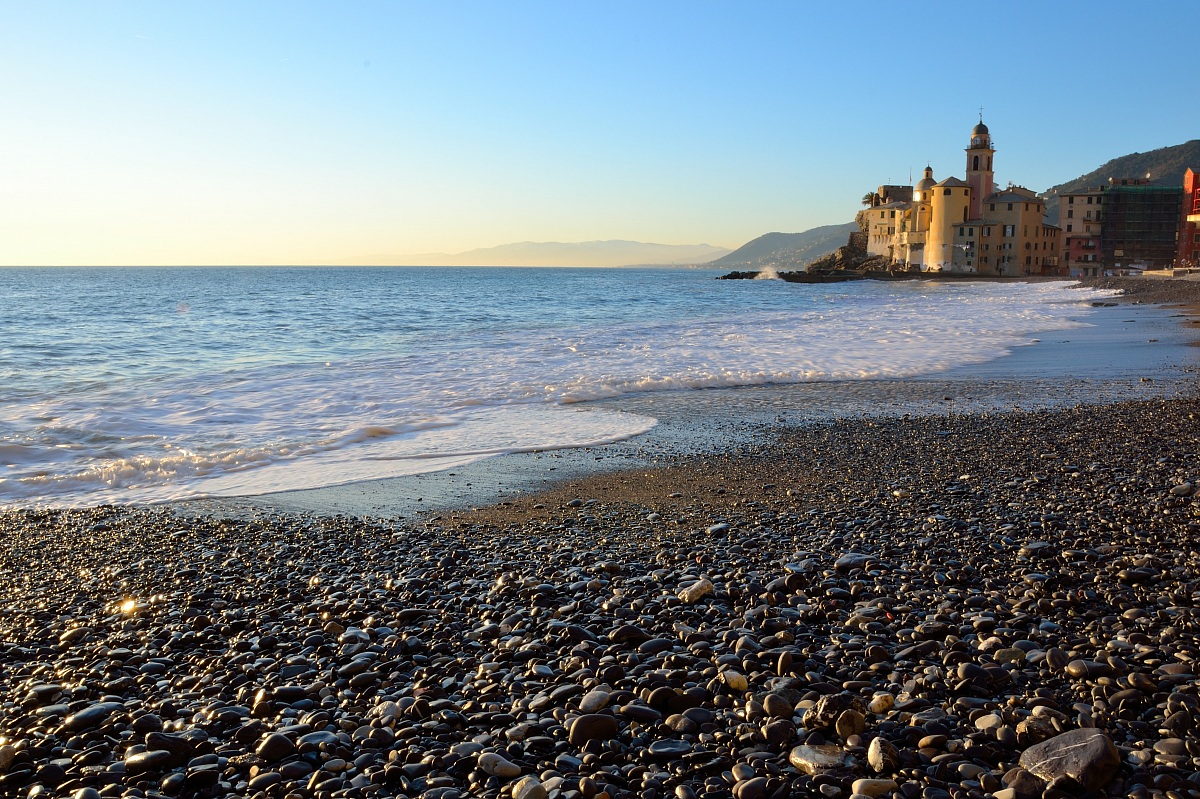
\includegraphics[scale=0.345]{./paqft.jpg}
}
%
\pgfsetfillopacity{0.8}%
%
\begin{frame}%
\bf
\vspace*{30pt}
%
\begin{exampleblock}{\vspace*{-3ex}}%
%
\begin{center}%
%
\Large Perturbative Algebraic Quantum Field Theory \\[10pt] on Curved Spacetime
%
\end{center}%
%
\end{exampleblock}%
%
\end{frame}
%
}%

%----------------------------------------------------------------------------%

\begin{frame}[label=input]

\frametitle{Physical input \hfill \hyperlink{details_input}{\beamergotobutton{details}} \qquad}

\vfill

\begin{itemize}
  
\item $(\Mcal,\gsf)$ : \textbf{4 dimensional} spacetime \\
\vspace*{8pt} $\to$ \ globally hyperbolic smooth manifold with Lorentzian metric \\[2pt]

\vfill

\item \textbf{Off shell} configuration space : \textbf{real scalar field} \\
\vspace*{8pt} $\to$ \ \textbf{space of real valued smooth maps} : $\phi \in \Ccal^\infty(\Mcal,\Rbb)$ \\[2pt]

\vfill

\item \textbf{Space of observables} : $\Fcal(\Mcal)$ 
%
\begin{equation*}
\ \Fsf : \left\{
\begin{array}{ccc}
\Ccal^\infty(\Mcal,\Rbb) & \to & \Cbb \\
\phi & \mapsto & \Fsf(\phi)
\end{array}
\right.
\end{equation*}
%
\textbf{Need to make restriction} to have good working properties\\[2pt]
%
\vspace*{8pt} $\to$ \ \textbf{support} and \textbf{regularity} properties

\end{itemize}

\vfill

\end{frame}  

%----------------------------------------------------------------------------%

\begin{frame}[label=obs]

\frametitle{Observables as functionals}

\vfill

\begin{itemize}

\item Observables : complex valued functionals

\item \textbf{Compactly supported} functionals : $\Fcal_0(\Mcal)$ \hfill \hyperlink{details_obs}{\beamergotobutton{definition}}

\item \textbf{Smooth} functionals : possible to compute functional derivatives at all orders

$\to$ \ Gâteaux derivatives \hfill \hyperlink{details_obs}{\beamergotobutton{functional derivative}}

\begin{example}
\vspace*{-25pt}
\begin{equation*}
\Fsf(\phi) = \int_\Mcal \dsf x \ \frac{\lambda}{4!} \ f(x) \ \phi(x)^4 \ , \ \ \  \Fsf^{(1)}(\phi)[\psi] =  \int_\Mcal \dsf x \ \frac{\lambda}{3!} \ f(x) \ \phi(x)^3 \ \psi(x)
\vspace*{-10pt}
\end{equation*}
\end{example}

\item functionals derivatives : distributions \\
$\to$ \ need to have \textbf{``regularity'' under control} $\to$ \textbf{wave front set}

\end{itemize}

\vfill

\end{frame}

%----------------------------------------------------------------------------%

\begin{frame}[label=wf]

\frametitle{Wave front set}

\vfill

\begin{block}{Definition -- Wave front set. \ \citebeam{Hörmander 1983} \hfill \hyperlink{details_wf}{\beamergotobutton{wave front set}}}
\vspace*{-8pt}
The wave front set $\WF(u) \subset T^\ast\Mcal^n$ of $u \in \Ccal^\infty_0(\Mcal^n)^\prime$ as follows \\
\qquad \textbf{(i)} \ for every $x \in \Mcal^n$ where $u$ is singular, choose a non-vanishing test function $f \in \Ccal^\infty_0(\Mcal^n)$ \\
\qquad \textbf{(ii)} \ $(x,k) \in \WF(u)$ iff $\hat{fu}(k)$ is \textbf{not} rapidly decreasing in the direction of $k \neq 0$ for some $f$.
\end{block}

$\to$ \ \textbf{local} and \textbf{covariant} under coordinate transformations.

\vfill

\begin{block}{Microlocal analysis. \citebeam{Hörmander 1983}}
\vspace*{-8pt}
The \textbf{pointwise product} of two distributions $u$, $v$ is well defined if 
\vspace*{-10pt}
\begin{equation*}
\WF(u) \oplus \WF(v) \neq 0 \ \Rightarrow \ \exists! \ u.v \in \Ccal^\infty_0(\Mcal^n)^{\prime} 
\vspace*{-8pt}
\end{equation*}
\end{block}

\vfill 

\end{frame}

%----------------------------------------------------------------------------%

\begin{frame}

\frametitle{Classical free field theory}

\vfill

\begin{itemize}

\item Equation of motion : \textbf{generalized Klein Gordon} equation
%
\vspace*{-8pt}
\begin{equation*} 
\Psf \phi = \left( \Box + \xi R + m^2 \right) \phi = 0
\vspace*{-8pt}
\end{equation*}
%
$\Mcal$ : \textbf{globally hyperbolic} spacetime $\to$ Cauchy problem well posed
\vspace*{-8pt}

\item \textbf{Fundamental solutions} $\Delta_{\rsf / \asf}$ \ $\to$ \ \textbf{causal propagator} of $\Psf$
\vspace*{-8pt}
%
\begin{equation*}
\Delta = \Delta_\rsf - \Delta_\asf \ , \quad \mbox{thus} \qquad \Psf_x \Delta(x,y) = 0
\vspace*{-8pt}
\end{equation*}

\item \textbf{Off shell} algebra

\begin{definition}[Classical free off shell algebra]
\vspace*{-5pt}
We define the classical free off shell algebra as follows
%
\vspace*{-5pt}
\begin{equation*}
\Acal_\reg(\Mcal) = \left(\Fcal_\reg(\Mcal), ^\ast , \cdot\right) \ , \ \ \mbox{with}
\vspace*{-5pt}
\end{equation*}
%
\begin{equation*}
\Fcal_{\mathsf{reg}}(\Mcal) = \left\{ \Fsf(\phi) \ \bigg| \ \Fsf(\phi) \in \Fcal_0(\Mcal) \ \mbox{ is smooth}, \ \Fsf^{(n)}(\phi) \in \Ccal^\infty_0(\Mcal^{n}) \right\} \ .
\vspace*{-5pt}
\end{equation*}
%
The involution is defined as $\Fsf^\ast(\phi) = \overline{\Fsf(\phi)}$, where $\overline{\cdot}$ is the complex conjugation.
%
\end{definition}

\end{itemize}

\end{frame}

%----------------------------------------------------------------------------%

\begin{frame}

\frametitle{Quantization of regular observables}

\vfill

\textbf{Classical} and \textbf{quantum observables} : \\
in the same vector space endowed with \textbf{different products} $\to$ different algebras
%
\vspace*{-10pt}
\begin{equation*}
\Acal_\reg(\Mcal)[[\hbar]] \quad \underset{\hbar \to 0}{\longrightarrow} \quad \Acal_\reg(\Mcal) \ . 
\vspace*{-8pt}%
\end{equation*}

\vfill

\textbf{``quantum regular observable''} : $\Fcal_\reg(\Mcal)[[\hbar]]$ 

\vfill

\begin{definition}[Quantum free regular off shell algebra]
\vspace*{-8pt}
We define it as a noncommutative, unital, associative $\ast$--algebra as follows
%
\vspace*{-10pt}
\begin{equation*}
\Acal_\reg(\Mcal)[[\hbar]] = \left(\Fcal_\reg(\Mcal)[[\hbar]] , ^\ast , \star \right) \ , \ \ \mbox{with}
\vspace*{-8pt}
\end{equation*}
%
\begin{equation*}
(\Fsf \star \Gsf)(\phi) = \Fsf(\phi) \cdot \Gsf(\phi) + \sum_{n=1}^\infty \frac{\hbar^n}{n!} \sm{ \Fsf^{(n)} , \Delta_+^{\otimes n} \Gsf^{(n) } } \ ,
\vspace*{-5pt}%
\end{equation*}
%
where $\Delta_+$ is a bidistribution, its antisymmetric part is the causal propagator, i.e. $i \Delta(x,y) = \Delta_+(x,y) - \Delta_+(y,x)$. This product is associative. 
\end{definition}

\vfill

$\to$ \ \textbf{noncommutative product} : implements canonical commutation relations

$\to$ \ \textbf{freedom} : symmetric part of $\Delta_+$ $\to$ \ isomorphic algebras

$\to$ \ \textbf{off shell}, but $\star$ product depends on the equation of motion with $\Delta_+$

\vfill

\end{frame}  

%----------------------------------------------------------------------------%

\begin{frame}

\frametitle{Enlarged spaces of observables}
  
\vfill  

\begin{exampleblock}{Hadamard condition \citebeam{Radzikowski 1996}}
\vspace*{-25pt}
\begin{equation*}
\WF(\Delta_+) \ = \ \bigg\{ (x,k_x ; y,-k_y) \in T^\ast\Mcal^2 \backslash \{0\} \ \bigg| \ (x,k_x) \sim (y,k_y) , \ k_x \triangleright 0 \bigg\}
\vspace*{-10pt}
\end{equation*}
$\sim$ : $\exists$ a null geodesic connecting $x$ and $x^\prime$, and $k^\prime$ is the parallel transport of $k$. \\
$k_x \triangleright 0$ : $k_x$ is future directed
\end{exampleblock}

\begin{itemize}

\item \textbf{Microcausal} functionals $\Fcal_{\mu\csf}(\Mcal)$
%
\vspace*{-5pt}
\begin{equation*}
\Fcal_{\mu\csf}(\Mcal) = \left\{ \Fsf(\phi) \ \bigg| \ 
\begin{array}{l}
\Fsf(\phi) \in \Fcal_0(\Mcal),  \ \Fsf^{(n)}(\phi) \in \Ecal^\prime(\Mcal^{\otimes n}), \\
\WF(\Fsf^{(n)}) \cap \left( \Mcal^n \times ( \overline{V^{n}_{+}} \cup \overline{V^{n}_{-}} ) \right)  = \emptyset 
\end{array}
\right\}
\vspace*{-7pt}
\end{equation*}
%
$\leadsto$ \textbf{pointwise product} of $\Delta_+$ : \textbf{well defined !} 
%
\vspace*{-5pt}
\begin{equation*}
\WF(\Delta_+) \oplus \WF(\Delta_+) \neq 0
\vspace*{-7pt}
\end{equation*}

\item \textbf{Interactions} $\to$ \textbf{Local} functionals $\Fcal_\loc(\Mcal)$ 
%
\vspace*{-7pt}
\begin{equation*}
\Fcal_\loc(\Mcal) := \left\{ \Fsf(\phi) \in \Fcal_{\mu\csf}(\Mcal) \ \bigg| \ \supp\left(\Fsf^{(n)}(\phi)\right) \subset d_n = \left\{ (x,\dots,x) \subset \Mcal^n \right\} \right\}
\vspace*{-7pt}
\end{equation*}
%
\end{itemize}

\vfill

\end{frame}  

%----------------------------------------------------------------------------%

\begin{frame}
 
\frametitle{``Regular'' time ordered product}

\vfill 

\textbf{Perturbation} of the free theory to \textbf{build} the \textbf{interacting theory}

\vfill

\textbf{Causal factorization property}
%
\vspace*{-8pt}
\begin{equation*}
\Fsf \cdot_\Tsf \Gsf = 
\left\{
\begin{array}{ll}
\Fsf \star \Gsf \quad \mbox{if } \ \supp(\Fsf) \ \mbox{ is later than  } \ \supp(\Gsf)  \\
\Gsf \star \Fsf \quad \mbox{if } \ \supp(\Gsf) \ \mbox{ is later than  } \ \supp(\Fsf) 
\end{array}
\right. 
\vspace*{-12pt}
\end{equation*}

\vfill

\begin{definition}[Regular time ordered product]
\vspace*{-8pt}
The time ordered product on $\Fcal_\reg(\Mcal)[[\hbar]]$ is defined as follows
%
\vspace*{-10pt}%
\begin{equation*}
(\Fsf \cdot_\Tsf \Gsf)(\phi) = \Fsf(\phi) \cdot \Gsf(\phi) + \sum_{n=1}^\infty \frac{\hbar^n}{n!} \sm{ \Fsf^{(n)} , \Delta_\fsf^{\otimes n} \Gsf^{(n) } } \ ,
\vspace*{-10pt}%
\end{equation*}
%
where $\Delta_\fsf$ is a time ordered version of $\Delta_+$, i.e. : $\Delta_\fsf(x,y) = \Theta(t_x-t_y) \Delta_+(x,y) + \Theta(t_y-t_x) \Delta_+(y,x)$.
\end{definition}

\vfill 

\end{frame}

%----------------------------------------------------------------------------%

\begin{frame}

\frametitle{Bogoliubov formula -- Interacting algebra}

$\bullet$ \ \textbf{Bogoliubov formula}\par
%
$\to$ \ \textbf{represents} the \textbf{interacting algebra} on the \textbf{free algebra}
%
\vspace*{-8pt}
\begin{equation*}
\Rsf_\Vsf(\Fsf) = S(\Vsf)^{\star-1} \star \left( S(\Vsf) \cdot_\Tsf \Fsf \right)
\vspace*{-8pt}
\end{equation*}
%
\begin{equation*}
\mbox{with} \ \ S(\Vsf) = \exp_\Tsf\left(\Vsf\right) = \sum^\infty_{n=0} \frac{i^n}{n!\ \hbar^n} \ \underbrace{\Vsf(\phi) \cdot_\Tsf \cdots \cdot_\Tsf \Vsf(\phi)}_{n \mbox{ times }} 
\vspace*{-2pt}
\end{equation*}

$\to$ \ ``interacting products'' in terms of the ``free products''
%
\vspace*{-7pt}
\begin{equation*}
\Fsf \star_{\mathsf{int}} \Gsf = \Rsf_\Vsf^{-1}\left( \Rsf_\Vsf(\Fsf) \star_{\mathsf{free}} \Rsf_\Vsf(\Gsf)\right)
\vspace*{-7pt}
\end{equation*}
%
$\to$ \  $\Rsf_\Vsf\left(\Fsf_\mathsf{lin}\left(\Psf\phi + \Vsf^{(1)}(\phi)\right)\right) = \Fsf_\mathsf{lin}(\Psf\phi) , \ \ \ \Fsf_\mathsf{lin}(\phi) = \mathlarger{\int_{\Mcal}} \dsf x \ \phi(x) \ f(x)$

\vfill
\vspace*{4pt}

$\bullet$ \ \textdbend \ \textbf{``Causal functionals''} $\Fcal_\Tsf(\Mcal)$ : time ordered products of $\Fcal_\loc(\Mcal)$ \\

\vfill

\begin{proposition}[Interacting quantum algebra]
%
\vspace*{-20pt}
\begin{equation*}
\Rsf_\Vsf \ : \ \Rcal_\Tsf(\Mcal)[[\hbar]] \ \to \ \Acal_\Tsf(\Mcal)[[\hbar]]
\end{equation*}
%
\vspace*{-20pt}
\begin{equation*}
\mbox{with} \ \ \Acal_\Tsf(\Mcal)[[\hbar]] = \left(\Fcal_\Tsf(\Mcal)[[\hbar]] , ^\ast , \star . \cdot_\Tsf \right) 
\vspace*{-6pt}
\end{equation*}
%
\end{proposition}

\end{frame}

%----------------------------------------------------------------------------%

\begin{frame}

\frametitle{First insight of our future problem}

\vfill

\begin{exampleblock}{Time ordered product \ \textdbend}
\vspace*{-15pt}
\begin{equation*} 
(\Fsf \cdot_\Tsf \Gsf)(\phi) = \Fsf(\phi) \cdot \Gsf(\phi) + \sum_{n=1}^\infty \frac{\hbar^n}{n!} \sm{\Fsf^{(n)}(\phi), \Delta_{\fsf}^{\otimes n} \Gsf^{(n)}(\phi)} 
\vspace*{-8pt}
\end{equation*}
\end{exampleblock}

\begin{center}
$\to$ powers of $\Delta_\fsf$ \textbf{ill defined} \ \textdbend
\end{center}

\vfill

$\leadsto$ \textbf{looking for} a time ordered product satisfying a \textbf{set of axioms}
\vspace*{-10pt}
%
\begin{multicols}{2}
\begin{itemize}
\setlength\itemsep{-2pt}
\item[T1 -- Initial condition.] 
\item[T2 -- Symmetry.]
\item[T3 -- Unitarity.]
\item[T4 -- Causal factorization.]
\item[T5 -- Field independence.]
\item[T6 -- Locality and covariance.]
\item[T7 -- Microlocal spectrum condition.] 
\hspace*{-13pt} $\dots$
\end{itemize}
\end{multicols}
\hfill\citebeam{Hollands \& Wald}

\vfill

\end{frame} 

%----------------------------------------------------------------------------%

{%
\setbeamertemplate{footline}{} 
\setbeamertemplate{headline}{}
\setbeamertemplate{background}{
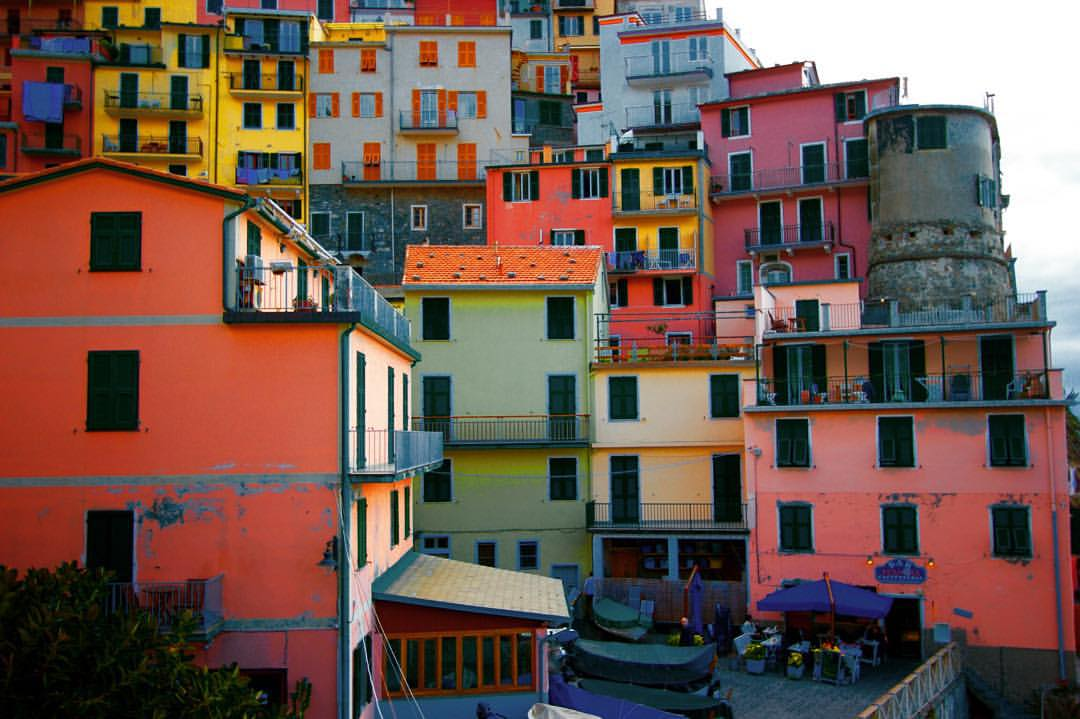
\includegraphics[scale=0.5]{./dimregcst.jpg}
}
%
\pgfsetfillopacity{0.8}%
%
\begin{frame}%
\bf
\vspace*{30pt}
%
\begin{exampleblock}{\vspace*{-3ex}}%
%
\begin{center}%
%
\Large A Covariant Regularization Scheme
%
\end{center}%
%
\end{exampleblock}%
%
\end{frame}
%
}%

%----------------------------------------------------------------------------%

\begin{frame}[label=sd]

\frametitle{``Characterizing'' divergences}

\vfill

\begin{definition}
\vspace*{-10pt}
\begin{itemize}
\setlength\itemsep{2pt}

\item $\exte{u} \in \Dcal^\prime(\Mcal^n)$ : \textbf{extension} of $u \in \Dcal^\prime\left(\Mcal^n \setminus d_n \right)$ \textbf{if} $\exte{u}(\phi) = u(\phi)$

\item $\left\{ u^{(\alpha)} \in \Dcal^\prime(\Mcal^n) \right\}$ : \textbf{analytic regularization} of a distribution, s.t.\\[2pt]
$u^{(\alpha)}$ weakly analytic w.r.t $\alpha \in \Omega \setminus \{0\}\subset \Cbb$, and $\underset{\alpha\to 0}{\lim} u^{(\alpha)} = u$

\end{itemize}
\vspace*{-8pt}
\end{definition}

\vspace*{-3pt}
$\to$ \ \textbf{total diagonal} : $d_n = \left\{ (x,\dots,x) \in \Mcal^n \right\}$

\vfill

\begin{exampleblock}{Extension using an analytic regularization}
\vspace*{-22pt}
\begin{equation*}
\exte{u} = \lim_{\alpha \to 0} \left( 1 - \pp \right) u^{(\alpha)} \quad \textdbend
\vspace*{-7pt}
\end{equation*}
\end{exampleblock}

\vspace*{-4pt}
$\to$ \ $\pp \left(u^{(\alpha)}\right)$ is supported in $d_n$, and poles in $\alpha$ of finite orders

\vfill

$\bullet$ \ The \textbf{scaling degree} of $u$ towards $d_n$ is defined as \hfill \hyperlink{details_sd}{\beamergotobutton{scaling degree}}
%
\vspace*{-5pt}
\begin{equation*}
\sd(u) \ := \ \inf\left\{ \omega \in \Rbb \ \left| \ \lim_{\lambda \downarrow 0} \ \lambda^\omega \ u_\lambda \ = \ 0 \right\} \right.
\vspace*{-8pt}
\end{equation*}

\begin{block}{Corollary \hfill \citebeam{Brunetti \& Fredenhagen (2000)}}
\vspace*{-6pt}
\textbf{If} \ $\sd(u) < 4(n-1)$, \textbf{then} $\exists ! \ \exte{u}$ towards $d_n$ with \textbf{same scaling degree}.
\end{block}

\vfill
 
\end{frame}

%----------------------------------------------------------------------------%

\begin{frame}[label=graph]

\frametitle{The Regularization problem}

\vfill

\textbf{Problem} : \textbf{extending} $\cdot_\Tsf$ to \textbf{local functionals}
%
\vspace*{-7pt}
\begin{equation*}
\Tcal_n \ : \ 
\left\{
\begin{array}{lcl}
\Fcal_\loc(\Mcal)[[\hbar]]^{\otimes n} & \to & \Fcal_\Tsf(\Mcal)[[\hbar]] \\
\Fsf_1 \otimes \ ... \ \otimes \Fsf_n & \mapsto & \msf_\nsf \circ \Tsf_n \bigg( \Fsf_1 \otimes \ ... \ \otimes \Fsf_n \bigg)
\end{array}
\right. 
\vspace*{-7pt}
\end{equation*}

\vfill

\textbf{Graphical view} :

$\to$ \ $\Gcal_n$ : set of graphs $\gamma$ with $n$ vertices, with $\ell_{ii}=0$ \\
\hspace*{13pt} $\ell_{ij}$ : number of edges between vertices $x_i$ and $x_j$ \hfill \hyperlink{details_graph}{\beamergotobutton{details}}
%
\begin{eqnarray*}
\Tsf_n \ = \ \sum_{\gamma \in \Gcal_n} \Tsf_\gamma \ , \ \ \mbox{with} \quad \Tsf_\gamma \ = \ \frac{1}{\Nsf(\gamma)} \ \sm{\tsf_\gamma \ , \ \delta_\gamma}
\end{eqnarray*}
%
\vspace*{-10pt}
%
\begin{eqnarray*}
&& \tsf_\gamma = \prod_{(i,j)\in\gamma} \Delta_\fsf(x_i,x_j)^{\ell_{ij}}
\quad \mbox{powers of } \ \Delta_\fsf \ \mbox{ : \textbf{ill defined!}} \quad \textdbend \\
&& \sd\left(\Delta_\fsf(x_i,x_j)^{\ell_{ij}}\right) = 2 \ell_{ij} , \ \mbox{unique extension for only } \ell_{ij} < 2 
\end{eqnarray*}

\vspace*{-2pt}
\vfill

\begin{exampleblock}{Example}
\vspace*{-29pt}
\begin{equation*}
\Fsf \cdot_{\Tsf} \Gsf  = \ \FG + \hbar \FoneG + \hbar^2 \FtwoG + \hbar^3 \FthreeG + \Ocal(\hbar^4)
\vspace*{-6pt}
\end{equation*}
\end{exampleblock}

\vfill

\end{frame}

%----------------------------------------------------------------------------%


\begin{frame}

\frametitle{Strategy}

\vfill

$\bullet$ \ $\tsf_\gamma$ \ : \ well defined \textbf{outside} of all \textbf{partial diagonals}, namely on $\Dcal(\Mcal^n\setminus D_n)$
%
\vspace*{-5pt}
\begin{equation*}
D_n = \left. \bigg\{x_1, \dots , x_n \ \right| \ x_i = x_j \ \text{ for at least one pair } \  (i,j), \ \mbox{ with } , \ i\neq j \bigg\} 
\vspace*{-20pt}
\end{equation*}
%
\begin{exampleblock}{Problem}
\vspace*{-14pt}
\begin{center}
Extend $\tsf_\gamma$ to $\Dcal(\Mcal^n)$ 
\end{center}
\vspace*{-5pt}
\end{exampleblock}


\vfill

$\bullet$ \ \textbf{Regularized expression} 
%
\vspace*{-7pt}
\begin{equation*}
\tsf^{(\alphabd)}_\gamma = \prod_{(i,j) \in \gamma} \Delta_\fsf(x_i,x_j)^{(\alpha_{ij},\ell_{ij})}
\vspace*{-7pt}
\end{equation*}

$\bullet$ \ \textbf{Principal part} : supported in partial diagonals $D_n$ \\
\hspace*{8pt} $\to$ \ subtraction in a recursive way : \textbf{Epstein Glaser forest formula}\\
\hspace*{24pt} starting from $D_2$ and proceeding with an increasing number of vertices

\vfill

$\bullet$ \ Extension : \textbf{method to compute principal parts}

\vfill

\begin{exampleblock}{Extension}
\vspace*{-14pt}
\begin{center}
$\left(\tsf_\gamma\right)_\ms = \underset{\alphabd \to 0}{\lim} \left(1-\pp\right)\tsf^{(\alphabd)}_\gamma $
\end{center}
\vspace*{-5pt}
\end{exampleblock}

\vfill

\end{frame}

%----------------------------------------------------------------------------%

\begin{frame}[label=forest]

\frametitle{Forest formula \& Minimal Subtraction}

\vfill

\begin{block}{Theorem -- Regularized time ordered product in the MS scheme \hfill \citebeam{Keller, \dots}}
\vspace*{-12pt}
%
\begin{equation*}
\Tcal_n = \left(\Tcal_n\right)_\ms = \lim_{\alphabd \to 0} \msf_\nsf \circ \left( \sum_{F\in\Frak_{\overline{n}}} \prod_{I\in F} \Rsf_I \right) \circ \Tsf^{(\alphabd)}_n
\end{equation*}
%
\begin{itemize}
\setlength\itemsep{0pt}
\item $\Rsf_I$ : ``\textbf{principal part operator}'' \ $\to$ \ if $I\subset J$, $\Rsf_I$ applied before $\Rsf_J$
%
\vspace*{-7pt}
\begin{equation*}
\Rsf_I \Tsf^{(\alphabd)}_n = - \pp_{\alphabd_I} \Tsf^{(\alphabd)}_n \ , \ \mbox{ with } \ \ \alphabd_I = \{\alpha_{ij}\}_{i,j \in I} \ , \ \ \mbox{ if } \ I=\emptyset \ , \quad \Rsf_\emptyset = \Ibb
\vspace*{-8pt}
\end{equation*}
%
\item before applying $\Rsf_I$ we set $\alpha_{ij}=\alpha_I$ for $i,j\in I$ 
%
\item $\alpha_{I} = \alpha_F$ for $I \in F$ before taking the sum over all forests \hfill \hyperlink{details_forest}{\beamergotobutton{definition}}
%
\item then $\alpha_F \to 0$
\end{itemize}
%
\end{block}

\vspace*{-20pt}

\begin{eqnarray*}
\FtwoGoneHoneF \hspace*{-10pt}
&& \tsf_\gamma^{(\alphabd)} = \Delta_\fsf(x_1,x_2)^{(\alpha_{12},2)} \ \Delta_\fsf(x_1,x_3) \ \Delta_\fsf(x_2,x_3) \\[-4pt]
&& \mbox{divergent contributions : } \{1,2\} \ \mbox{and} \ \{1,2,3\} \\[-2pt]
&& \mbox{relevant forests : } \{\emptyset\} \ , \ \ \{\{1,2\}\} \ , \ \ \{\{1,2,3\}\} \ , \ \ \{\{1,2\},\{1,2,3\}\} \\[-2pt]
&& \mbox{regularized } \tsf_\gamma \ : \ \left(\tsf_\gamma\right)_\ms = 
\lim_{\alphabd \to 0} \left(1+\Rsf_{12}+\Rsf_{123}+\Rsf_{123}\Rsf_{12}\right) \tsf^{(\alphabd)}_\gamma
\end{eqnarray*}

\vfill

\end{frame}

%----------------------------------------------------------------------------%

\begin{frame}

\frametitle{Explicit forms}

\vfill

\begin{block}{Hadamard form}
\vspace*{-25pt}
\begin{eqnarray*}
&& \Delta_\fsf(x,y) = \lim_{\epsilon \downarrow 0} \ \frac{1}{8\pi^2}\left(\frac{u(x,y)}{\sigma_\fsf(x,y)}+v(x,y) \ \log(M^2 \sigma_\fsf(x,y))+w(x,y)\right)  \\
&& \sigma_\fsf(x,y) = \sigma(x,y) + i\epsilon 
\vspace*{-8pt}
\end{eqnarray*}
$\to$ \ $\sigma(x,y)$ : half squared geodesic distance \\ 
$\to$ \ $u,v,w$ smooth (Hadamard coefficients)
\end{block}

\vfill

we recall $\tsf_\gamma^{(\alphabd)}$ :
%
\vspace*{-20.5pt}
\begin{eqnarray*}
\qquad \tsf^{(\alphabd)}_\gamma &=& \prod_{(i,j) \in \gamma} \Delta_\fsf(x_i,x_j)^{(\alpha_{ij},\ell_{ij})} \\[-2pt]
\qquad \Delta_\fsf^\alpha &=& \lim_{\epsilon \downarrow 0} \ \frac{1}{8\pi^2}\left(\frac{u}{\sigma_\fsf^{1+\alpha}} + \frac{v}{\alpha} \ \left( 1 - \frac{1}{\sigma_\fsf^\alpha}\right) \right) + w  
\vspace*{-5pt}
\end{eqnarray*}

\vfill

\textbf{Relevant part} in $\tsf_\gamma^{(\alphabd)}$ :
%
\vspace*{-5pt}
\begin{equation*}
\Asf_\gamma^{\alphabd} = \prod_{(i,j)\in\gamma} \frac{1}{\sigma_\fsf^{\ell_{ij}(1+\alpha_{ij})}}
\vspace*{-7pt}
\end{equation*}

\vfill

\textbf{Building blocks} :
%
\vspace*{-5pt}
\begin{equation*}
\frac{1}{\sigma_\fsf^\alpha}
\end{equation*}

\vfill

\end{frame}

%----------------------------------------------------------------------------%

\begin{frame}[label=homog]

\frametitle{Important properties}

\vfill

\begin{proposition}
$\Ncal \subset\Mcal^2$ geodesically convex space, $\alpha \in \Cbb$, $\phi \in \Ccal^\infty_0(\Ncal)$
%
\begin{equation*}
\sm{ \frac{1}{\sigma^\alpha_\fsf} , \phi } = \lim_{\epsilon \to 0^+ } \ \int_{\Mcal^2} \dsf x \ \dsf y \ \frac{1}{(\sigma(x,y)+i\epsilon)^{\alpha}} \ \phi(x,y)
\end{equation*}
%
\begin{itemize}
\setlength\itemsep{2pt}
%
\item It is a distribution which is analytic in $\alpha$ on $\Ccal^\infty_0(\Ncal\setminus d_2)$
%
\item It is homogeneous of degree $-2\alpha$ \hfill \hyperlink{details_homog}{\beamergotobutton{details}}
%
\item It is a well defined distribution on $\Ccal^\infty_0(\Ncal)$ for $2\alpha-4 \notin \Nbb$
%
\item Its smearing product is analytic for $2\alpha-4 \notin \Nbb$, and meromorphic in $\alpha$ with simple poles at $2\alpha-4\in \Nbb$
%
\end{itemize}
%
\end{proposition}

\vfill

\begin{proposition}
\vspace*{-4pt}
$\sm{\Asf_\gamma^{(\alphabd)},\phi}$ is an \textbf{analytic} function in every $\alpha_{ij}$, with $\alphabd = \{\alpha_{ij}\}$ and $\phi\in\Ccal^\infty_0\left(\Mcal^n\setminus D_n\right)$
\end{proposition}

\vfill

\end{frame}

%----------------------------------------------------------------------------%

\begin{frame}[label=theorem]

\frametitle{Extension}

\vfill

\begin{block}{Theorem}
\vspace*{-5pt}
$\Asf_\gamma^{(\alphabd)}$ can be extended from $\Mcal^n\setminus D_n$ to $\Mcal^n$
\end{block}

\vfill

\begin{itemize}
\setlength\itemsep{-1pt}

\item $\Asf_\gamma^{(\alphabd)}$ : sum of \textbf{homogeneous distributions} plus a \textbf{remainder} towards the total diagonal $d_n$
%
\vspace*{-7pt}
\begin{equation*}
\Asf_\gamma^{(\alphabd)} = \sum_{k=1}^m \ \Asf_{\gamma,k}^{(\alphabd)} + r_\gamma^{(\alphabd)}
\vspace*{-7pt}
\end{equation*}
%
$\to$ \ $r_\gamma^{(\alphabd)}$ has lower scaling degree than $\Asf_\gamma^{(\alphabd)}$

\item isolate the poles \hfill \hyperlink{details_theorem}{\beamergotobutton{details}}
%
\vspace*{-5pt}
\begin{equation*}
\rho \Asf_\gamma^{(\alphabd)} = - \sum_{(i,j)\in\gamma} 2 \ell_{ij}(1+ \alpha_{ij}) \Asf_\gamma^{(\alphabd)} + r^{(\alphabd)}_\gamma
\vspace*{-5pt}
\end{equation*}
%
with $\rho$ a differential operator built in terms of $\sigma$ and $\nabla$ 

\end{itemize}

\vfill

\hfill \hyperlink{details_theorem_ex}{\beamergotobutton{example}}

\end{frame}

%----------------------------------------------------------------------------%

\begin{frame}

\frametitle{Properties of the scheme}

\vfill
 
\begin{exampleblock}{Theorem}
\vspace*{-4pt}
This regularization scheme satisfies the axioms we asked before.
\end{exampleblock}
 
\vfill 

In particular 

\begin{itemize}
\item $\Tcal_n$ satisfies the causal factorization

\item $\Tcal_n$ is local and covariant

\item If the spacetime $\Mcal$ has non trivial isometries and if $\Delta_\fsf$ is chosen such as to be invariant under these isometries, then $\Tcal_n$ is invariant under these isometries as well
\end{itemize}


\vfill
 
\end{frame}

%----------------------------------------------------------------------------%

{
\setbeamertemplate{footline}{} 
\setbeamertemplate{headline}{}
\setbeamertemplate{background}{
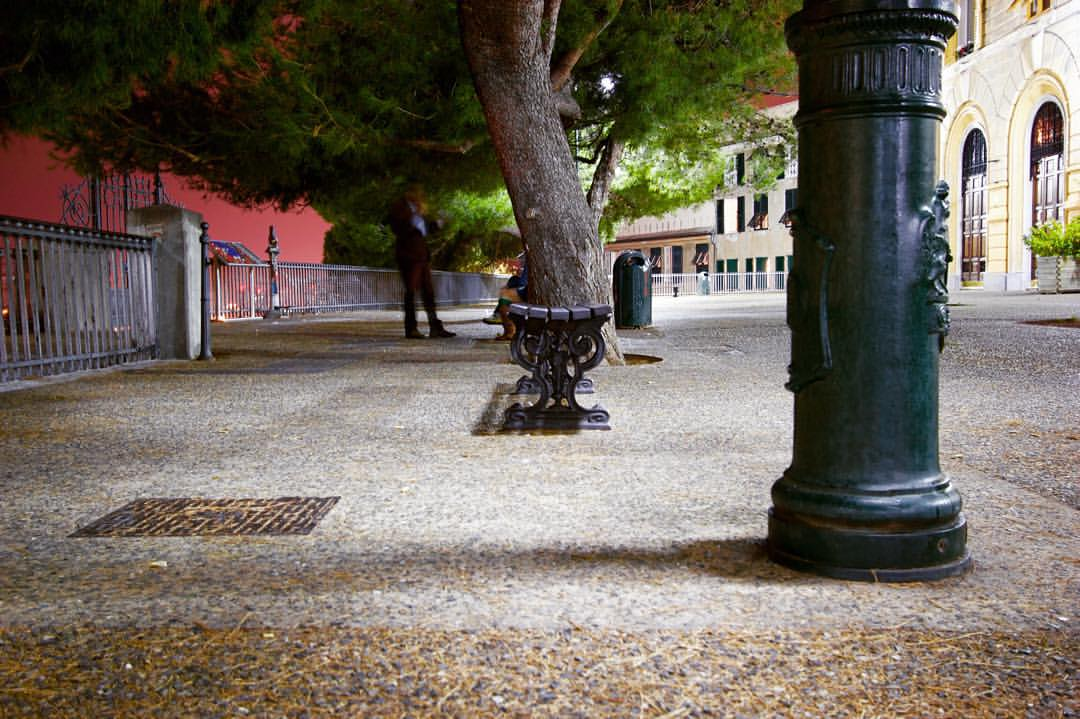
\includegraphics[width=\paperwidth,height=\paperheight]{flrw.jpg}
}
\pgfsetfillopacity{0.8}
\begin{frame}
\bf
\begin{exampleblock}{\vspace*{-3ex}}
\begin{center}
\Large Explicit computations on spatially flat \\[10pt] Friedmann Lemaître Robertson Walker spacetimes
\end{center}
\end{exampleblock}
\end{frame}
}

%----------------------------------------------------------------------------%

\begin{frame}[label=flrw]
 
\frametitle{Spatially flat FLRW spacetime} 

\begin{itemize}
\setlength\itemsep{4pt} 
 
\item \textbf{spatially flat Friedmann Lemaître Robertson Walker} spacetime
%
\vspace*{-5pt}
\begin{equation*}
g = a(\tau)^2 \ \left( - d\tau^2 + d\vec{x}^2 \right) 
\vspace*{-5pt}
\end{equation*}
%
$\to$ \ our scheme is invariant under the isometries of FLRW spacetime

\begin{block}{Goal :}
\vspace*{-20pt}
\begin{center}
Compute the fish diagram : \FtwoG \ $\to$ \ $(\Delta_\fsf)^2$ 
\end{center}
\end{block}
\vspace*{-5pt}

\item \textbf{in principle} we can compute all quantities in spatial and momentum space

\item \textdbend \quad however even for spatially flat FLRW spacetimes, \\
$\sigma, u, v, w$ are \textbf{not explicitly known} neither in \textbf{position space}, nor in \textbf{momentum space}

\item \textbf{Idea}: $\Delta_\fsf=\Delta_{\fsf,0}+\delta \Delta_\fsf$, with \\[3pt]

$\to$ $\Delta_{\fsf,0}$ contains sufficiently many singular contributions \\[3pt]

$\to$ $\Delta_{\fsf,0}$ explicitly known in position and momentum space

\end{itemize}

\end{frame}

%----------------------------------------------------------------------------%

\begin{frame}

\frametitle{Fish diagram for FLRW} 

$\bullet \ \Delta_{\fsf,0} \to$ the \textbf{Feynman propagator} of the \textbf{massless}, \textbf{conformally coupled} $(\xi = \frac16)$ \textbf{Klein Gordon field} in the conformal vacuum
%
\begin{equation*}
\Delta_{\fsf,0}(x_1,x_2)=\frac{1}{8\pi^2 a(\tau_1)a(\tau_2)}\frac{1}{\sigma_{\Mbb}(x_1,x_2)+i\epsilon} 
\end{equation*}

$\bullet \ $ Fish diagram
\vspace*{-12pt}
\begin{equation*}
(\Delta_\fsf)^2_\ms = (\Delta_{\fsf,0})^2_\ms + 2 \delta\Delta_\fsf \Delta_{\fsf,0} + (\delta\Delta_\fsf)^2
\vspace*{-25pt}
\end{equation*}

\begin{eqnarray*}
(\Delta_{\fsf,0})^2_\ms &=& 
\lim_{\alpha\to 0} \left( 1 - \pp \right) \frac{1}{M^{2\alpha}} (\Delta_{\fsf,0})^{2+\alpha} \\
&=& - \frac{1+2\log(a)}{16\pi^2 a^4} i\delta_\Mbb-\frac{1}{2(8\pi^2)^2 a^2\otimes a^2} \left(\Box_{\Mbb}\otimes 1\right)\frac{\log{M^2\sigma_{\epsilon,\Mbb}}}{\sigma_{\epsilon,\Mbb}}
\end{eqnarray*}

and then compute the Fourier transform \dots

\end{frame}

%----------------------------------------------------------------------------%

{
\setbeamertemplate{footline}{} 
\setbeamertemplate{headline}{}
\setbeamertemplate{background}{
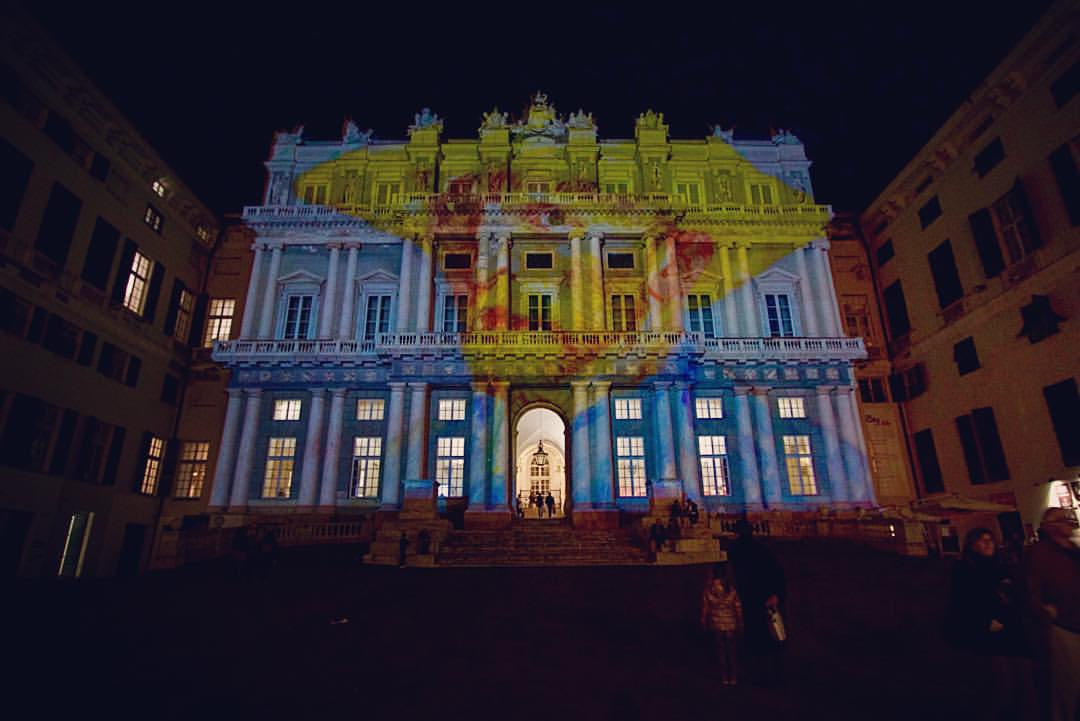
\includegraphics[width=\paperwidth,height=\paperheight]{grazie.jpg}
}
\begin{frame}
\vspace*{220pt}
\textcolor{white!80!blue}{\bf \LARGE Grazie.}
\end{frame}
}

%----------------------------------------------------------------------------%

\appendix
\backupbegin

%----------------------------------------------------------------------------%

\begin{frame}[label=details_input]

\frametitle{Spacetime \& configuration space}

\vfill

\begin{definition}[Curved spacetime]
A pair $(\Mcal,g)$ is a \textbf{curved spacetime} if $\Mcal$ is a $4$ dimensional \textbf{Lorentzian manifold}, endowed with a Lorentzian metric of signature $( - + \dots +)$, required to be orientable, paracompact, time orientable, and \textbf{globally hyperbolic}. 
\end{definition}

\vfill

\begin{definition}[Off shell configuration space]
The off shell configuration space over the spacetime $\Mcal$ is the \textbf{space of real valued smooth maps}, $\phi \in \Ccal^\infty(\Mcal,\Rbb)$. It is equipped with the locally convex topology.
\end{definition}

\vfill

\hfill\hyperlink{input}{\beamerreturnbutton{back}}
  
\end{frame}

%----------------------------------------------------------------------------%

\begin{frame}[label=details_obs]

\frametitle{Analysis}

\vfill

\begin{block}{Spacetime support of $\Fsf$}
\vspace*{-15pt}
\begin{equation*}
\supp(\Fsf) \doteq \left\{ x \in \Mcal \bigg| 
\begin{array}{l} 
\forall \ \mbox{neighborhood } U \mbox{ of } x, \ \exists \ \phi, \psi \in \mbox{ smooth}, \\
\supp(\psi) \subset U, \mbox{ such that } \Fsf(\phi + \psi) \neq \Fsf(\phi).
\end{array}
\right\}
\end{equation*}
\end{block}

\vfill

\begin{definition}[Smooth functional]
\vspace*{-5pt}
The $n$-th derivative of a functional $\Fsf$ at $\phi \in \Usf$ with respect to the directions $\psi_1, \dots, \psi_n \in \Ccal^\infty(\Mcal)$ is defined as a map $\Fsf : \Usf \times \Ccal^\infty(\Mcal)^{\otimes n} \to \Ccal^\infty(\Mcal)$,
%
\begin{equation*}
\Fsf^{(n)}(\phi)[\psi_1,\dots ,\psi_n] =  \lim_{t \to 0} \ \frac{1}{t} \bigg( \Fsf^{(n-1)}(\phi + t \psi_n) \ - \ \Fsf^{(n-1)}(\phi) \bigg)[\psi_1,\dots ,\psi_{n-1}] \ .
\end{equation*}
%
The map $\Fsf$ is said to be \textbf{smooth} at $\phi \in \Usf$ if \hfill\hyperlink{joint_cont}{\beamerreturnbutton{details}}\\
%
$\bullet$ \ the limit exists for all $\psi_1, \dots, \psi_n \in \Ccal^\infty(\Mcal,\Rbb)$,\\
$\bullet$ \ and if $\Fsf^{(n)}$ is jointly continuous on the product space $\Usf \times \Ccal^\infty(\Mcal,\Rbb)^{\otimes n}$.\\ 
%
\end{definition}

\vfill


\vfill

\hfill\hyperlink{obs}{\beamerreturnbutton{back}}

\end{frame}

%----------------------------------------------------------------------------%

\begin{frame}[label=joint_cont]

\frametitle{Jointly continuous map}

\vfill

We recall that a map 
%
\begin{equation*}
\fsf : \Usf \times \Xsf \to \Ysf
\end{equation*}
%
is \textbf{jointly continuous} at $(x,y) \in \Xsf \times \Usf$, if 
%
\begin{eqnarray*}
&& \mbox{for each neighborhood} \ \Ysf^\prime \ \mbox{of} \ \fsf(x,y) \ , \\
&& \exists \ \mbox{a product of open sets} \ \Usf^\prime \times \Xsf^\prime \subseteq \Usf \times \Xsf \ \mbox{containing} \ (x,y) \ , \\
&& \mbox{such that} \ \fsf(\Usf^\prime \times \Xsf^\prime) \subseteq \Ysf^\prime \ .
\end{eqnarray*}

\vfill

\hfill\hyperlink{details_obs}{\beamerreturnbutton{back}}

\end{frame}

%----------------------------------------------------------------------------%

\begin{frame}[label=details_wf]

\frametitle{Wave front set}

\vfill

\textbf{Examples} : \\ 

$\leadsto$ \ $\WF(\delta) = \left\{ (0,k) | k \in \Rbb^n , k \neq 0 \right\} $ \\
\textit{Proof}: The singular support of $\delta(x)$ is $\{0\}$ and $\hat{f\delta}(k) = f(0)$ is not fast decreasing if $f(0) = 0$. \\[12pt]

$\leadsto$ 
\vspace*{-17pt}
\begin{equation*}
\hspace*{-110pt} u(x) = \frac{1}{x^2 + i \epsilon}, \quad \WF(u) = \{ (0;k) | k<0 \}
\end{equation*}
\textit{Proof}: By contour integration $\hat{u}(k) = -2i\pi \Theta(-k)$, thus
\begin{equation*}
\abs{\hat{fu}(k)} = \abs{ \frac{1}{2\pi} \int_\Rbb dq \ \hat{f}(q) \ \hat{u}(k-q) } = \abs{ \int_k^\infty dq \ \hat{f}(q) }
\end{equation*}
\qquad Fourier transform of a test function, $\hat{f}(q)$, is fast decreasing for $q \geq 0$ !!

\vfill


\hfill\hyperlink{wf}{\beamerreturnbutton{back}}

\end{frame}

%----------------------------------------------------------------------------%

\begin{frame}[label=details_sd]

\frametitle{Scaling degree}

$\bullet$ \ $\exists !$ geodesic $\gamma_i$ connecting $x_1$ and $x_i$
%
\vspace*{-8pt}
\begin{equation*}
\gamma_i : \lambda \mapsto \gamma_i(\lambda) = x_i(\lambda) \ , \ \mbox{ with } \ x_i(0) =x_1, \ x_i(1) = x_i
\vspace*{-8pt}
\end{equation*}
%
$\bullet$ \ \textbf{geometric scaling transformation} 
%
\vspace*{-8pt}
\begin{equation*}
\phi_\lambda = \lambda^{4(n-1)} \ \phi\left(x_1(\lambda ),x_2(\lambda ),\dots,x_n(\lambda\right)) \ \prod_{i=2}^n \sqrt{\abs{\frac{g(x_i(\lambda ))}{g(x_i)}}}
\vspace*{-8pt}
\end{equation*}
%
where $g(x)$ is the determinant of the metric $g$

\vfill

$\bullet$ \ \textbf{scaled distributions} 
%
\vspace*{-8pt}
\begin{equation*}
\sm{u_\lambda,\phi} := \sm{u,\phi_{1/\lambda}} 
\vspace*{-8pt}
\end{equation*}
% 
$\bullet$ \ $\WF(u)$ is \textbf{transversal} to $d_n$ if 
%
\vspace*{-8pt}
\begin{equation*}
\overline{\WF(u)}\cap \left\{(x_1,\dots, x_n,k,0,\dots,0)\in T^*\Mcal^n, \forall k\neq 0 \right\} = \emptyset 
\vspace*{-8pt}
\end{equation*}

\vfill

$\bullet$ \ Definition of $\mathcal{D}^\prime_\Gamma(\Mcal^n\setminus d_n)$
%
\vspace*{-8pt}
\begin{equation*}
\mathcal{D}^\prime_\Gamma(\Mcal^n\setminus d_n) = \left\{ u \in \mathcal{D}^\prime(\Mcal^n\setminus d_n) \ , \ \WF(u) \subset \Gamma \right\}
\vspace*{-8pt}
\end{equation*}

\vfill

\hfill\hyperlink{sd}{\beamerreturnbutton{back}}
 
\end{frame}

%----------------------------------------------------------------------------%

\begin{frame}[label=details_graph]

\frametitle{Graphical analysis}

\vfill

\begin{eqnarray*}
&& \Tsf_n \ = \ \sum_{\gamma \in \Gcal_n} \Tsf_\gamma \ , \qquad \mbox{with} \quad \Tsf_\gamma \ = \ \frac{1}{\Nsf(\gamma)} \ \sm{\tsf_\gamma \ , \ \delta_\gamma} \\
%
&& \Nsf(\gamma) = \hbar^{-\abs{\Esf(\gamma)}} \prod_{(i,j) \in \gamma} \abs{\ell_{ij}} ! \ , \quad 
%
\delta_\gamma = \frac{\delta^{2\abs{E(\gamma)}}\hfill}{\underset{(i,j)\in\gamma}{\prod} \delta \phi_i^{\abs{\ell_{ij}}}} \ , \quad 
%
\tsf_\gamma = \prod_{(i,j)\in\gamma} \Delta_{ij}^{\abs{\ell_{ij}}} 
%
\vspace*{-5pt}
\end{eqnarray*}

\vfill

\begin{eqnarray*}
(\Fsf \cdot_{\Tsf} \Gsf \cdot_{\Tsf} \Ksf)(\phi)
&=& \FGH+\hbar\left(\FoneGHF+\FGoneHF+\FGHoneF\right) \\
&&+\hbar^2\left[\FoneGHoneF+\FoneGoneHF+\FGoneHoneF\right.\\
&&\left.+\frac12\left(\FtwoGHF+\FGtwoHF+\FGHtwoF\right)\right]
+\mathcal{O}(\hbar^3)
\end{eqnarray*}

\vfill

\hfill\hyperlink{graph}{\beamerreturnbutton{back}}

\end{frame}

%----------------------------------------------------------------------------%

\begin{frame}[label=details_forest]

\frametitle{Forest formula}

\vfill

\textbf{Epstein Glaser forest formula}\\
\hspace*{5pt} (this method does not depend on the graph expansion)

$\bullet$ \ \textbf{set of indices}
%
\vspace*{-5pt}
\begin{equation*}
\overline{n} := \{1,\dots , n\}
\vspace*{-5pt}
\end{equation*}
%
$\bullet$ \ \textbf{forest} $F$ : a collection of subsets of $\overline{n}$ 
%
\vspace*{-5pt}
\begin{equation*}
F = \{ I_1,\dots, I_k\} \ , \qquad I_j \subset \overline{n} \ , \qquad \mbox{and} \qquad \abs{I_j} \geq 2
\vspace*{-5pt}
\end{equation*}
%
we require
%
\vspace*{-5pt}
\begin{equation*}
I_i\cap I_j = \emptyset \ , \qquad \text{or} \qquad I_i \subset I_j \ , \qquad \mbox{or} \qquad  I_j\subset I_j
\vspace*{-5pt}
\end{equation*}
%
$\mathfrak{F}_{\overline{n}}$ : the \textbf{set of all forests} of $n$ indices together with the empty forest $\{\emptyset\}$.

\vfill

\hfill\hyperlink{forest}{\beamerreturnbutton{back}}
 
\end{frame}

%----------------------------------------------------------------------------%

\begin{frame}[label=details_homog]

\frametitle{Homogeneous distribution}

\vfill

\begin{definition}
A distribution $u \in \Dcal^\prime(\Mcal^n)$ or $u\in \Dcal^\prime(\Mcal^n\setminus d_n)$, which satisfies the equality 
%
\vspace*{-5pt}
\begin{equation*}
\lambda^{\delta} \sm{ u , \phi_\lambda } = \sm{ u , \phi } \ , \quad \forall \lambda > 0 \ , 
\vspace*{-5pt}
\end{equation*}
%
under geometric scaling transformations for all $\phi\in\Dcal(\Ncal_n\setminus d_n)$ and for a $\delta\in\Cbb$, is called \textbf{homogeneous of degree} $\delta$. 
\end{definition}

\vfill

\begin{equation*}
\inf\bigg\{ \omega \in \Rbb \ \bigg| \ \lim_{\lambda \downarrow 0} \lambda^\omega \sm{u,\phi_{1/\lambda}} = \lim_{\lambda \downarrow 0} \lambda^{\omega+\Re(\delta)} \lambda^{i\Im(\delta)} \sm{u,\phi}
= 0  \bigg\} = - \Re(\delta) \ ,
\end{equation*}

\vfill

\hfill\hyperlink{homog}{\beamerreturnbutton{back}}

\end{frame}

%----------------------------------------------------------------------------%

\begin{frame}[label=details_theorem]

\frametitle{Euler operator}
\vfill

\vspace*{-5pt}
\begin{equation*}
u^{(\alpha)}  = \sum_{k=0}^m u^{(\alpha)}_k + r^{(\alpha)}
\vspace*{-5pt}
\end{equation*}
%
where $u^{(\alpha)}_k$ are homogeneous, with degree with degree $a_k = - \delta_\alpha + k$
%
\vspace*{-5pt}
\begin{equation*}
\sd(u^{(\alpha)}_k) = - \Re(a_k)  =\Re\left(\delta_\alpha\right) - k \geq 4(n-1)
\vspace*{-5pt}
\end{equation*}
%
Euler operator
%
\vspace*{-5pt}
\begin{equation*}
\Esf_p : \left\{
\begin{array}{lcl}
\Dcal(\Ncal_n) & \to & \Dcal(\Ncal_n) \\
\phi(x_1,\dots, x_n) & \mapsto & \left. (-1)^p \ \lambda^{p+4(n-1)} \ \dfrac{d^p}{d\lambda^p} \bigg( \lambda^{-4(n-1)}  \phi_\lambda(x) \bigg) \right|_{\lambda = 1}
\end{array}
\right.
\vspace*{-5pt}
\end{equation*}
%
we have
%
\vspace*{-5pt}
\begin{equation*}
\sm{ u^{(\alpha)}_k, \phi } = \frac{1}{\overset{p-1}{\ \underset{j=0}{\prod}} \ (a_k+j+4(n-1))}   \sm{ u^{(\alpha)}_k, \Esf_p \phi }
\vspace*{-5pt}
\end{equation*}

\vfill

\hfill\hyperlink{theorem}{\beamerreturnbutton{back}}

\end{frame}

%-----------------------------------------------------------------------------%

\begin{frame}[label=details_theorem_ex]

\frametitle{The fish diagram ($2$ vertices)}

\vfill

\begin{minipage}{0.2\linewidth}
\centering
\begin{figure}
\begin{tikzpicture}[thick,scale=0.5] 
\filldraw (-1,0) circle (1pt) node[left] {$x$};
\filldraw (1,0) circle (1pt) node[right] {$y$};
\draw (0,0) circle (1cm and 0.6cm);
\end{tikzpicture}
\end{figure}
\end{minipage}
\hspace*{-8pt}
$\longrightarrow$
\hspace{5pt}
\begin{minipage}{0.7\linewidth}
\vspace*{-13pt}
\begin{equation*}
\Delta_\fsf^2(x,y) = \frac{1}{8 \pi^2} \bigg( \frac{u^2(x,y)}{\sigma_\fsf^2(x,y)} +  
\mbox{``well defined for $x=y$''}
\bigg)
\end{equation*}
\end{minipage}

\vspace*{20pt}

$\bullet$ regularize only $\sigma_\fsf^{-(2+\alpha)}$ \\

$\bullet$ use $\sigma$ identities : \ $ \Box \sigma = 4 + f \sigma $ \\
 
$\bullet$ $\alpha \mapsto \sigma_\fsf^{-(2+\alpha)}$ (weakly) meromorphic in $\alpha$. \\
\quad $\to$ Laurent series w.r.t $\alpha$ \\
\quad $\to$ subtract the principal part and take the limit $\alpha \to 0$
 
\begin{equation*}
\left(\frac{1}{\sigma_\fsf^2}\right)_\ms\ = \ \lim_{\alpha \to 0} \ \left( 1 - \pp \right) \frac{1}{\sigma_\fsf^{2+\alpha}} 
\end{equation*}
\begin{equation*}
\Longrightarrow \ \left(\Delta_\fsf^{2}\right)_\ms
\end{equation*}

\vfill

\hfill\hyperlink{theorem}{\beamerreturnbutton{back}}

\end{frame}

%-----------------------------------------------------------------------------%

\backupend

%============================================================================%
\end{document} 
%============================================================================%